% Preambel mit Einstellungen importieren
% Document type and used packages
\documentclass[open=right, % Kapitel darf nur auf rechten Seite beginnen
    paper=A4,               % DIN-A4-Papier
    a4paper,                % DIN-A4-Papier
    12pt,                   % Schriftgöße
    headings=small,         % Kleine Überschriften
    headsepline=true,       % Trennlinie am Kopf der Seite
    footsepline=false,      % Keine Trennlinie am Fuß der Seite
    bibliography=totoc,     % Literaturverzeichnis in das Inhaltsverzeichnis aufnehmen
    twoside=on,             % Doppelseitiger Druck - auf off stellen für einseitig
    DIV=7,                  % Verhältnis der Ränder zum bedruckten Bereich
    chapterprefix=true,     % Kapitel x vor dem Kapitelnamen
    cleardoublepage=plain]{scrbook} 

% Pakete einbinden, die benötigt werden
\usepackage{scrpage2}
\usepackage[utf8]{inputenc}       	% Dateien in UTF-8 benutzen
\usepackage[T1]{fontenc}          	% Zeichenkodierung
\usepackage{graphicx}             	% Bilder einbinden
\usepackage[ngerman,english]{babel} % Deutsch und Englisch unterstützen
\usepackage{xcolor}               	% Color support
\usepackage{amsmath}              	% Matheamtische Formeln
\usepackage{amsfonts}             	% Mathematische Zeichensätze
\usepackage{amssymb}              	% Mathematische Symbole
\usepackage{float}                	% Fließende Objekte (Tabellen, Grafiken etc.)
\usepackage{booktabs}             	% Korrekter Tabellensatz
\usepackage[printonlyused]{acronym} % Abkürzungsverzeichnis [nur verwendete Abkürzugen]
\usepackage{makeidx}              	% Sachregister
\usepackage{listings}             	% Source Code listings
%\usepackage{minted}                 % https://www.overleaf.com/learn/latex/Code_Highlighting_with_minted
\usepackage{listingsutf8}         	% Listings in UTF8
\usepackage[hang,font={sf,footnotesize},labelfont={footnotesize,bf}]{caption} % Beschriftungen
\usepackage[scaled]{helvet}       	% Schrift Helvetia laden
\usepackage[absolute]{textpos}	  	% Absolute Textpositionen (für Deckblatt)
\usepackage{calc}                 	% Berechnung von Positionen
\usepackage{blindtext}            	% Blindtexte
\usepackage[bottom=40mm,left=35mm,right=35mm,top=30mm]{geometry} % Ränder ändern
\usepackage{setspace}             	% Abstände korrigieren
\usepackage{ifthen}               	% Logische Bedingungen mit ifthenelse
\usepackage{scrhack}              	% Get rid of tocbasic warnings
\usepackage[pagebackref=false]{hyperref}  % Hyperlinks
\usepackage[all]{hypcap}          	% Korrekte Verlinkung von Floats
\usepackage[autostyle=true,german=quotes]{csquotes}   % Zitate
\usepackage[backend=biber,
  isbn=false,                     	% ISBN nicht anzeigen, gleiches geht mit nahezu allen anderen Feldern
  %sortlocale=de_DE,               	% Sortierung der Einträge für Deutsch
  sortlocale=en_US,              	% Sortierung der Einträge für Englisch
  autocite=inline,                	% regelt Aussehen für \autocite (inline=\parancite)
  hyperref=true,                  	% Hyperlinks für Ziate
  style=ieee                     	% Zitate als Zahlen [1]
  %style=alphabetic               	% Zitate als Kürzel und Jahr [Ein05]
  %style=authoryear                	% Zitate Author und Jahr [Einstein (1905)]
]{biblatex}                       	% Literaturverwaltung mit BibLaTeX
\usepackage{rotating}             	% Seiten drehen
\newcommand\tabrotate[1]{\begin{turn}{90}\rlap{#1}\end{turn}}
\newcommand\tabhightadjust[1][-.75\normalbaselineskip]{\hspace{#1}}
\usepackage{subfigure}			% Mehrere Bilder in einem
\usepackage{tikz}			% Flow charts
\usetikzlibrary{shapes,positioning}	% Flow charts position
\usepackage{pgfplots}			% Function plots
\usepackage{array,multirow}		% Rotation of text in tables
\usepackage{xspace}			% Space after Trademark sign
\usepackage{svg}			% include svgs

\usetikzlibrary{matrix, positioning}	% matrix in tikz

\newfont{\chess}{chess20}
\newfont{\bigchess}{chess30}
\newcommand{\chf}{\baselineskip20pt\lineskip0pt\chess}

\setlength{\bibitemsep}{1em}     	% Abstand zwischen den Literaturangaben
\setlength{\bibhang}{2em}        	% Einzug nach jeweils erster Zeile

% Trennung von URLs im Literaturverzeichnis (große Werte [> 10000] verhindern die Trennung)
\defcounter{biburlnumpenalty}{10} 	% Strafe für Trennung in URL nach Zahl
\defcounter{biburlucpenalty}{500}  	% Strafe für Trennung in URL nach Großbuchstaben
\defcounter{biburllcpenalty}{500}  	% Strafe für Trennung in URL nach Kleinbuchstaben

% Farben definieren
\definecolor{linkblue}{RGB}{0, 0, 100}
\definecolor{linkblack}{RGB}{0, 0, 0}
\definecolor{comment}{RGB}{63, 127, 95}
\definecolor{darkgreen}{RGB}{14, 144, 102}
\definecolor{darkblue}{RGB}{0,0,168}
\definecolor{darkred}{RGB}{128,0,0}
\definecolor{javadoccomment}{RGB}{0,0,240}

% Einstellungen für das Hyperlink-Paket
\hypersetup{
    colorlinks=true,      % Farbige links verwenden       
%    allcolors=linkblue,
    linktoc=all,          % Links im Inhaltsverzeichnis
    linkcolor=linkblack,  % Querverweise
    citecolor=linkblack,  % Literaturangaben
	filecolor=linkblack,  % Dateilinks
	urlcolor=linkblack    % URLs
}

% Einstellungen für Quelltexte
\lstset{     
      xleftmargin=0.2cm,     
      basicstyle=\footnotesize\ttfamily,
      keywordstyle=\color{darkgreen},
      identifierstyle=\color{darkblue},
      commentstyle=\color{comment}, 
      stringstyle=\color{darkred}, 
      tabsize=2,
      lineskip={2pt},
      columns=flexible,
      inputencoding=utf8,
      captionpos=b,
      breakautoindent=true,
	  breakindent=2em,
	  breaklines=true,
	  prebreak=,
	  postbreak=,
      numbers=none,
      numberstyle=\tiny,
      showspaces=false,      % Keine Leerzeichensymbole
      showtabs=false,        % Keine Tabsymbole
      showstringspaces=false,% Leerzeichen in Strings
      morecomment=[s][\color{javadoccomment}]{/**}{*/},
      literate={Ö}{{\"O}}1 {Ä}{{\"A}}1 {Ü}{{\"U}}1 {ß}{{\ss}}2 {ü}{{\"u}}1 {ä}{{\"a}}1 {ö}{{\"o}}1
}

\urlstyle{same}

% Einstellungen für Überschriften
\renewcommand*{\chapterformat}{%
  \Large\chapapp~\thechapter   % Große Schrift
  \vspace{0.3cm}               % Abstand zum Titel des Kapitels
}

% Abstände für die Überschriften setzen
\renewcommand{\chapterheadstartvskip}{\vspace*{2.6cm}}
\renewcommand{\chapterheadendvskip}{\vspace*{1.5cm}}

\RedeclareSectionCommand[
  beforeskip=-1.8\baselineskip,
  afterskip=0.25\baselineskip]{section}

\RedeclareSectionCommand[
  beforeskip=-1.8\baselineskip,
  afterskip=0.15\baselineskip]{subsection}

\RedeclareSectionCommand[
  beforeskip=-1.8\baselineskip,
  afterskip=0.15\baselineskip]{subsubsection}


% In der Kopfzeile nur die kurze Kapitelbezeichnung (ohne Kapitel davor)
\renewcommand*\chaptermarkformat{\thechapter\autodot\enskip}
\automark[chapter]{chapter}

% Einstellungen für Schriftarten
\setkomafont{pagehead}{\normalfont\sffamily}
\setkomafont{pagenumber}{\normalfont\sffamily}
\setkomafont{paragraph}{\sffamily\bfseries\small}
\setkomafont{subsubsection}{\sffamily\itshape\bfseries\small}
\addtokomafont{footnote}{\footnotesize}
\setkomafont{chapter}{\LARGE\selectfont\bfseries}

% Wichtige Abstände
\setlength{\parskip}{0.2cm}  % 2mm Abstand zwischen zwei Absätzen
\setlength{\parindent}{0mm}  % Absätze nicht einziehen
\clubpenalty = 10000         % Keine "Schusterjungen"
\widowpenalty = 10000        % Keine "Hurenkinder"
\displaywidowpenalty = 10000 % Keine "Hurenkinder"
\renewcommand{\footnotesize}{\fontsize{9}{10}\selectfont} % Größe der Fußnoten
\setlength{\footnotesep}{8pt} % Abstand zwischen den Fußnoten

% Index erzeugen
\makeindex

% Einfacher Font-Wechsel über dieses Makro
\newcommand{\changefont}[3]{
\fontfamily{#1} \fontseries{#2} \fontshape{#3} \selectfont}

% Eigenes Makro für Bilder
\newcommand{\bild}[3]{
\begin{figure}[h]
  \centering
  \includegraphics[width=#2]{#1}
  \caption{#3}
  \label{#1}
\end{figure}}

% Wo liegt Sourcecode?
\newcommand{\srcloc}{src/}

% Wo sind die Bilder?
\graphicspath{{img/}}

% Makros für typographisch korrekte Abkürzungen
\newcommand{\zb}[0]{z.\,B.\ }
\newcommand{\dahe}[0]{d.\,h.\ }
\newcommand{\ua}[0]{u.\,a.\ }

% Flags für Veröffentlichung und Sperrvermerk
\newboolean{dhbwpublizieren}
\newboolean{dhbwsperrvermerk}

% White space after trademark sign
\let\OldTexttrademark\texttrademark
\renewcommand{\texttrademark}{\OldTexttrademark\xspace}%


% Dokumenteninfos importieren
% -------------------------------------------------------
% Daten für die Arbeit
% Wenn hier alles korrekt eingetragen wurde, wird das Titelblatt
% automatisch generiert. D.h. die Datei titelblatt.tex muss nicht mehr
% angepasst werden.

\newcommand{\dhbwsprache}{en} % de oder en für Deutsch oder Englisch
                              % Für korrekt sortierte Literatureinträge, noch preambel.tex anpassen

% Titel der Arbeit auf Deutsch
\newcommand{\dhbwtitelde}{Animation des N-Damen Problems in JavaScript}

% Titel der Arbeit auf Englisch
\newcommand{\dhbwtitelen}{Animation of n-queens problem in JavaScript}

% Weitere Informationen zur Arbeit
\newcommand{\dhbwort}{Mannheim}    % Ort
\newcommand{\dhbwautorvname}{Koen} % Vorname(n)
\newcommand{\dhbwautornname}{Logmann} % Nachname(n)
\newcommand{\dhbwautorrvname}{Jessica} % Vorname(n)
\newcommand{\dhbwautorrnname}{Roth} % Nachname(n)
\newcommand{\dhbwdatum}{\today} % Datum der Abgabe
\newcommand{\dhbwjahr}{2019} % Jahr der Abgabe
\newcommand{\dhbwfirma}{} % Firma bei der die Arbeit durchgeführt wurde
\newcommand{\dhbwbetreuer}{Prof. Dr. Karl Stroetmann, DHBW Mannheim} % Betreuer an der Hochschule
\newcommand{\dhbwzweitkorrektor}{} % Betreuer im Unternehmen oder Zweitkorrektor
\newcommand{\dhbwfakultaet}{I} % I für Informatik
\newcommand{\dhbwstudiengang}{AI} % IB IMB UIB IM MTB

% Zustimmung zur Veröffentlichung
\setboolean{dhbwpublizieren}{true}   % Einer Veröffentlichung wird zugestimmt
\setboolean{dhbwsperrvermerk}{false} % Die Arbeit hat keinen Sperrvermerk

% -------------------------------------------------------
% Abstract

% Kurze (maximal halbseitige) Beschreibung, worum es in der Arbeit geht auf Deutsch
\newcommand{\dhbwabstractde}{TODO} %TODO

% Kurze (maximal halbseitige) Beschreibung, worum es in der Arbeit geht auf Englisch

\newcommand{\dhbwabstracten}{Todo} %TODO



% Literatur-Datenbank
\addbibresource{literatur.bib}   % BibLaTeX-Datei mit Literaturquellen einbinden

\begin{document}
\frontmatter

% Römische Ziffern für die "Front-Matter"
\setcounter{page}{0}
\changefont{ptm}{m}{n}  % Times New Roman für den Fließtext
\renewcommand{\rmdefault}{ptm}

% Titelblatt
% -------------------------------------------------------
% In dieser Datei sollten eigentlich keine Veränderungen mehr
% notwendig sein.
% -------------------------------------------------------

\thispagestyle{empty}

% Fakultäten der DHBW-Mannheim
% -------------------------------------------------------
\ifthenelse{\equal{\dhbwfakultaet}{I}}%
  {\newcommand{\dhbwfakultaetlangde}{Fakultät für Informatik}%
   \newcommand{\dhbwfakultaetlangen}{Department of Computer Science}}{}

\ifthenelse{\equal{\dhbwfakultaet}{E}}%
  {\newcommand{\dhbwfakultaetlangde}{Fakultät für Elektrotechnik}%
   \newcommand{\dhbwfakultaetlangen}{Department of Electrical Engineering}}{}

\ifthenelse{\equal{\dhbwfakultaet}{S}}%
  {\newcommand{\dhbwfakultaetlangde}{Fakultät für Sozialwesen}%
   \newcommand{\dhbwfakultaetlangen}{Department of Social Work}}{}



\ifthenelse{\equal{\dhbwstudiengang}{IB}}%
  {\newcommand{\dhbwstudienganglangde}{Informatik}%
  \newcommand{\dhbwstudienganglangen}{Computer Science}%
  \newcommand{\dhbwtypde}{Bachelor-Thesis}%
  \newcommand{\dhbwtypen}{Bachelor Thesis}%
  \newcommand{\dhbwgrad}{\dhbwbsc}}{}
  
\ifthenelse{\equal{\dhbwstudiengang}{AI}}%
  {\newcommand{\dhbwstudienganglangde}{Angewandte Informatik}%
  \newcommand{\dhbwstudienganglangen}{Applied Computer Science}%
  \newcommand{\dhbwtypde}{Bachelor-Thesis}%
  \newcommand{\dhbwtypen}{Bachelor Thesis}%
  \newcommand{\dhbwgrad}{\dhbwbsc}}{}

\ifthenelse{\equal{\dhbwstudiengang}{SAB}}%
  {\newcommand{\dhbwstudienganglangde}{Soziale Arbeit}%
   \newcommand{\dhbwstudienganglangen}{Social Labour}%
   \newcommand{\dhbwtypde}{Bachelor-Thesis}%
   \newcommand{\dhbwtypen}{Bachelor Thesis}%
   \newcommand{\dhbwgrad}{\dhbwba}}{}
   
\ifthenelse{\equal{\dhbwstudiengang}{SAM}}%
  {\newcommand{\dhbwstudienganglangde}{Soziale Arbeit}%
   \newcommand{\dhbwstudienganglangen}{Social Labour}%
   \newcommand{\dhbwtypde}{Master-Thesis}%
   \newcommand{\dhbwtypen}{Master Thesis}%
   \newcommand{\dhbwgrad}{\dhbwmastera}}{}

\ifthenelse{\equal{\dhbwstudiengang}{TIB}}%
  {\newcommand{\dhbwstudienganglangde}{Technische Informatik}%
   \newcommand{\dhbwstudienganglangen}{Technical Information Technology}%
   \newcommand{\dhbwtypde}{Bachelor-Thesis}%
   \newcommand{\dhbwtypen}{Bachelor Thesis}%
   \newcommand{\dhbwgrad}{\dhbwbsc}}{}
  

\newcommand{\dhbwbsc}{Bachelor of Science (B.Sc.)}
\newcommand{\dhbwba}{Bachelor of Arts (B.A.)}
\newcommand{\dhbwmaster}{Master of Science (M.Sc.)}
\newcommand{\dhbwmastera}{Master of Arts (M.A.)}
\newcommand{\dhbwmasterba}{Master of Business Administration (MBA)}

\newcommand{\dhbwkoerperschaftde}{DHBW Mannheim}
\newcommand{\dhbwkoerperschaften}{University of Applied Sciences Mannheim}

\newcommand{\dhbwautorbib}{\dhbwautornname, \dhbwautorvname \ \& \dhbwcoautornname, \dhbwcoautorvname} % Autor Nachname, Vorname
\newcommand{\dhbwautor}{\dhbwautorvname \ \dhbwautornname \ \& \dhbwcoautorvname \ \dhbwcoautornname} % Autor Vorname Nachname

\ifthenelse{\equal{\dhbwsprache}{de}}%
  {\newcommand{\dhbwtyp}{\dhbwtypde}%
   \newcommand{\dhbwthesistype}{zur Erlangung des akademischen Grades \dhbwgrad}%
   \newcommand{\dhbwkoerperschaft}{\dhbwkoerperschaftde}%
   \newcommand{\dhbwstudiengangname}{Studiengang \dhbwstudienganglangde}%
   \newcommand{\dhbwstudienganglang}{\dhbwstudienganglangde}%
   \newcommand{\dhbwtitel}{\dhbwtitelde}%
   \newcommand{\dhbwtutor}{Betreuer}%
   \newcommand{\dhbwfakultaetlang}{\dhbwfakultaetlangde}%
   \newcommand{\dhbwlistoftables}{Tabellenverzeichnis}%
   \newcommand{\dhbwlistoffigures}{Abbildungsverzeichnis}%
   \newcommand{\dhbwlistings}{Quellcodeverzeichnis}%
   \newcommand{\dhbwindex}{Index}%
   \newcommand{\dhbwabbreviations}{Abkürzungsverzeichnis}%   
   \selectlanguage{ngerman}}
   %else
  {\newcommand{\dhbwtyp}{\dhbwtypen}%
   \newcommand{\dhbwthesistype}{for the acquisition of the academic degree \dhbwgrad}%
   \newcommand{\dhbwkoerperschaft}{\dhbwkoerperschaften}%
   \newcommand{\dhbwstudiengangname}{Course of Studies: \dhbwstudienganglang}%
   \newcommand{\dhbwstudienganglang}{\dhbwstudienganglangen}%
   \newcommand{\dhbwtitel}{\dhbwtitelen}%
   \newcommand{\dhbwtutor}{Tutors}
   \newcommand{\dhbwfakultaetlang}{\dhbwfakultaetlangen}%
   \newcommand{\dhbwlistoftables}{List of Tables}%
   \newcommand{\dhbwlistoffigures}{List of Figures}%
   \newcommand{\dhbwlistings}{Listings}%
   \newcommand{\dhbwindex}{Index}%
   \newcommand{\dhbwabbreviations}{List of Abbreviations}%
   \selectlanguage{english}}%


% Daten in die Standard-Felder von KOMA-Script eintragen
\titlehead{\dhbwtyp\ in\  \dhbwstudienganglang}
\subject{}
\title{\dhbwtitel}
\author{\dhbwauthor}
\date{\small{\dhbwdatum}}

% Daten für das fertige PDF-Dokument
\hypersetup{
  pdftitle={\dhbwtitel},  % Titel des Dokuments
  pdfauthor={\dhbwautor},              % Autor
  pdfsubject={\dhbwtyp\ in\ \dhbwstudienganglang},                % Thema
  pdfkeywords={\dhbwtitel}         % Schlüsselworte
}

\newlength{\bindekorrektur}
\newlength{\seitenanfang}
\newlength{\seitenbreite}
  
\setlength{\bindekorrektur}{-46mm}   % Korrektur der horizontalen Position
\setlength{\seitenanfang}{0mm}       % Korrektur der vertikalen Position
\setlength{\seitenbreite}{297mm}

%\noindent
\includegraphics[width=7cm]{dhbw-logo.pdf}\\
\noindent
\includegraphics[width=0.49\textwidth]{img/DHBW-Logo.pdf}
\hfill
%\noindent\includegraphics[width=0.27\textwidth]{SAP_grad_R_pref.png}

% Titel der Arbeit
\begin{textblock*}{128mm}(45mm,\seitenanfang + 62mm) % 4,5cm vom linken Rand und 6,0cm vom oberen Rand
  \centering\Large\sffamily
  \vspace{4mm} % Kleiner zusätzlicher Abstand oben für bessere Optik
  \textbf{\dhbwtitel}
\end{textblock*}%

% Name
\begin{textblock*}{128mm}(45mm,\seitenanfang + 103mm)
  \centering\large\sffamily
  \dhbwautor
\end{textblock*}

% Thesis
\begin{textblock*}{\seitenbreite}(\bindekorrektur,\seitenanfang + 130mm)
  \centering\large\sffamily
  \dhbwtyp\\
  \begin{small}\dhbwthesistype \end{small}\\
  \vspace{2mm}
  \dhbwstudiengangname
\end{textblock*}

% Fakultät
\begin{textblock*}{\seitenbreite}(\bindekorrektur,\seitenanfang + 165mm)
  \centering\large\sffamily
  \dhbwfakultaetlang\\
  \vspace{2mm}
  \dhbwkoerperschaft
\end{textblock*}

% Datum
\begin{textblock*}{\seitenbreite}(\bindekorrektur,\seitenanfang + 190mm)
  \centering\large 
  \textsf{\dhbwdatum}
\end{textblock*}

% Firma
\begin{textblock*}{\seitenbreite}(\bindekorrektur,\seitenanfang + 215mm)
  \centering\large 
  %\textsf{Durchgeführt bei der Firma \dhbwfirma}
\end{textblock*}

% Betreuer
\begin{textblock*}{\seitenbreite}(\bindekorrektur,\seitenanfang + 240mm)
  \centering\large\sffamily
  \dhbwtutor \\
  \vspace{2mm}
  \dhbwbetreuer\\
  \vspace{2mm}
  \dhbwzweitkorrektor
\end{textblock*}

% Bibliographische Informationen
\null\newpage
\thispagestyle{empty}
  
\newcommand{\dhbwbibde}{\begin{small}\textbf{\dhbwautorbib}: \\ \dhbwtitelde \ / \dhbwautor. \ -- \\ \dhbwtypde, \dhbwort : \dhbwkoerperschaftde, \dhbwjahr. \pageref{lastpage} Seiten.\end{small}}

\newcommand{\dhbwbiben}{\begin{small}\textbf{\dhbwautorbib}: \\ \dhbwtitelen \ / \dhbwautor. \ -- \\ \dhbwtypen, \dhbwort : \dhbwkoerperschaften, \dhbwjahr. \pageref{lastpage} pages. \end{small}}

\ifthenelse{\equal{\dhbwsprache}{de}}%
  {\dhbwbibde \\ \vspace{0.5cm} \\ \dhbwbiben}
  {\dhbwbiben \\ \vspace{0.5cm} \\ \dhbwbibde}


% Erklärung
\clearpage\setcounter{page}{1}
\thispagestyle{empty}
\textsf{\large\textbf{Erklärung}}

Hiermit erkläre ich, dass ich die vorliegende Arbeit selbstständig verfasst und keine anderen als die angegebenen Quellen und Hilfsmittel benutzt habe.

\ifthenelse{\boolean{dhbwpublizieren} \and \not\boolean{dhbwsperrvermerk}}%
{
\vspace{0.5cm}
Ich bin damit einverstanden, dass meine Arbeit veröffentlicht wird, d.\,h. dass die Arbeit elektronisch gespeichert, in andere Formate konvertiert, auf den Servern der Hochschule Mannheim öffentlich zugänglich gemacht und über das Internet verbreitet werden darf. 
}{}%


\vspace{1cm}
\dhbwort, \dhbwdatum \\

\vspace{1.2cm}						                                      
\dhbwautor

\ifthenelse{\boolean{dhbwsperrvermerk}}%
{%
\vspace{11cm}
\color{red}\textsf{\large\textbf{Sperrvermerk}}

Diese Arbeit basiert auf internen und vertraulichen Daten des Unternehmens \dhbwfirma.

Diese Arbeit darf Dritten, mit Ausnahme der betreuenden Dozenten und befugten Mitglieder des Prüfungsausschusses, ohne ausdrückliche Zustimmung des Unternehmens und des Verfassers nicht zugänglich gemacht werden.

Eine Vervielfältigung und Veröffentlichung der Arbeit ohne ausdrückliche Genehmigung -- auch in Auszügen -- ist nicht erlaubt.
\color{black}
}{}

\cleardoublepage

% Abstract
\chapter*{Abstract}

\ifthenelse{\equal{\dhbwsprache}{de}}%
  {\subsubsection*{\dhbwtitelde}\dhbwabstractde\subsubsection*{\dhbwtitelen}\dhbwabstracten}
  {\subsubsection*{\dhbwtitelen}\dhbwabstracten\subsubsection*{\dhbwtitelde}\dhbwabstractde}



% Inhaltsverzeichnis erzeugen
\cleardoublepage
\pdfbookmark{\contentsname}{Contents}
\tableofcontents

% Korrigiert Nummerierung bei mehrseitigem Inhaltsverzeichnis
\cleardoublepage
\newcounter{frontmatterpage}
\setcounter{frontmatterpage}{\value{page}}

% Arabische Zahlen für den Hauptteil
\mainmatter

% Den Hauptteil mit vergrößertem Zeilenabstand setzen
\onehalfspacing

% ------------------------------------------------------------------
% Hauptteil der Arbeit
    % !TeX root = ./documentation.tex

\chapter{Introduction}
\label{ch:introduction}

\section{Motivation}
\label{sec:introMotivation}
% cSpell:disable
%TODO Koen: Fällt dir was besseres ein?
%Der Davis Putman Algorithmus ist ein wichtiges Werkzeug zur Lösung von bekannten mathematischen Problemen wie beispielsweise das N Damen Problem. Dies ist auch der Grund, weshalb dieser oftmals zum Erklären von aussagelogischen Prinzipien verwendet wird. Oftmals ist es aber schwierig nachzuvollziehen, wie der ALgorithmus aussagelogische Probleme löst, da es allein durch das Betrachten der Rechenwege des Algorithmus nur schwer zu verstehen ist.
%\\
%Wenn es die Möglichkeit gäbe, die Lösung des N Damen Problems Schritt für Schritt zu verfolgen und dies visuell veständlich angezeigt zu bekommen, dann würde dies viele Verständnisprobleme klären und den Lernprozess deutlich beschleunigen. Dies ist auch der Grund, weshalb dieses Programm zur Visualisieren des Davis Putman Algorithmus so wichtig ist. Es kann zu vielen Zwecken wie beispielsweise der Unterstützung von Lehrveranstaltungen verwendet werden und hilft damit vielen Interessierten einen einfachen Einstieg in diesen komplexen Algorithmus.
% cSpell:enable
The \textit{Davis-Putman algorithm} is an important tool for solving known mathematical problems such as the \textit{N-Queens Problem}. This is also the reason why it is often used to explain propositional logic principles. However, it is often difficult to understand how the algorithm finds possible solutions for propositional logic problems, as it is difficult to understand by just looking at the algorithm's computational paths.

If there would be the possibility to follow the solution of the \textit{N-Queens Problem} step by step with a visual representation of the current state, then this would clarify many understanding problems and enhance the learning process. This is also the reason why this program is so important for visualizing the Davis Putman algorithm. It can be used for many purposes, such as supporting lectures, and thus helps many interested people to easily get started with this complex algorithm.

\section{Objective of the work}
\label{sec:introObjective}
% cSpell:disable
%TODO Koen: Fällt dir noch etwas dazu ein?
%Die Aufgabenstellung dieser Studienarbeit handelt von der Animation des Davis Putman Algorithmus anhand des N Damen Problems mit der Hilfe von Javascript. Dabei werden mehrere Kriterien definiert, die diese Animation erfüllen muss, da sie vor allem zur Visualisierung und zur genaueren anschaulichen Verdeutlichung beziehungsweise Erklärung des Algorithmus dient. Die genauen Anforderungen werden im Laufe dieser Arbeit genauer spezifiziert und am Ende am finalen Produkt evaluiert. Der Hauptteil dieser Arbeit handelt deshalb von der Konzeption und der Implementierung dieser Aufgabenstellung.
% cSpell:enable
The task of this student research project is the animation of the \textit{Davis-Putman algorithm} on the basis of the \textit{N-Queens Problem} with the help of JavaScript. Several criteria are defined, which this animation must fulfill, since it serves above all for the visualization and for the more exact descriptive clarification and/or explanation of the algorithm. The exact requirements are specified more precisely in the course of this work and evaluated at the end of the final product. The main part of this work therefore deals with the conception and implementation of this task.

\section{Structure of the report}
\label{sec:introStructure}
% cSpell:disable
%Um die Navigation durch diese Arbeit zu erleichtern, wird im folgenden Abschnitt einen kurzen Blick in die Struktur dieser Arbeit geworfen. 
%\\
%Im nächsten Kapitel werden die mathematischen Grundlagen zum Davis Putman Algorithmus und des N Damen Problems geschaffen. Dabei handelt es sich vor allem um die logischen Zusammenhänge und der mathematisch korrekten Definition des zu lösenden Problems. 
%\\
%Darauffolgend wird im dritten Kapitel ein allgemeiner Überblick zu den verwendeten Bibliotheken und Technologien gegeben und Hintergrundinformationen geliefert, aus welchen Gründen bestimmte Technologien bevorzugt beziehungsweise ausgewählt wurden.
%\\
%Im vierten Abschnitt dieser Arbeit wird die Konzeption des Programms genauer betrachtet. Vor allem handelt es von der allgemeinen Architektur und dem erstellten Layout Design, das als Vorlage für die Implementierung der Benutzeroberfläche dient. Eingeleitet wird das Kapitel durch das Spezifizieren der Anforderungen für das Programm, die eine zentrale Rolle in der Evaluation am Ende spielen.
%\\
%Im fünften Kapitel wird nun Schritt für Schritt durch die fertige Implementierung geleitet und der Aufbau des Programms genauer erläutert. Dabei wird durch die unterschiedlichen Komponenten und Klassen geführt und dabei ihre Funktion genauer erläuert.
%\\
%Das letzte Kapitel wird mit der Evaluation der Anforderungen begonnen. Dies dient vor allem dazu, um zu schauen, ob das Programm alle Kriterien erfüllt und zu Ende als erfolgreich erfüllt angesehen werden kann. Danach folgt ein zusammenfassendes Fazit und ein Ausblick, wie das Programm zukünftig weiterentwickelt oder anders eingesetzt werden könnte.
% cSpell:enable
In order to facilitate navigation through this work, the following section takes a brief look at the structure of this work.

In the next chapter explains the scientific basics of the \textit{Davis-Putman algorithm} and the \textit{N-Queens Problem}. These are mainly about the logical correlations and the mathematically correct definition of the problem to be solved.

The third chapter then gives a general overview of the libraries and technologies used and provides background information on the reasons why certain technologies were preferred or selected.

The fourth section of this paper takes a closer look at the design of the program. It mainly deals with the general architecture and the created layout design, which serves as a template for the implementation of the user interface. The chapter is introduced by specifying the requirements for the program, which are mandatory for the evaluation at the end.

In the fifth chapter, step by step you will be guided through the finished implementation and the structure of the program will be explained in more detail. The different components and classes are guided through and their roles explained in more detail.

The last chapter starts with the evaluation of the requirements. This is mainly to see if the program meets all the criteria and can be considered successful at the end. This is followed by a summary and an outlook on how the program or its components could be further developed or used in other ways in the future.
    % !TeX root = ../documentation.tex

% Davis Putnam in own word

\chapter{Scientific Basics}
\label{ch:sciBasics}
% cSpell:disable
% Das Ziel dieser Arbeit besteht in der Visualisierung des \textit{Davis-Putman algorithm}us, der das sogenannte N damen Problem lösen soll. Dafür muss zuerst ein allgemeines Verständnis zu diesem Algorithmus und dem mathematischen Problem geschaffen werden. In diesem Kapitel wird aus diesem Grund dieses fundamentale Wissen zusammengefasst, um eine Basis für die weiterführende Entwicklung zu schaffen. Dafür spielt unter anderem die Deklarierung des mathematischen Problems eine Rolle, damit dieses vom \textit{Davis-Putman algorithm}us gelöst werden kann.
% cSpell:enable
The purpose of this work is to visualize the \textit{Davis-Putnam algorithm} solving the so-called \textit{N-Queens Problem}. Therefore a general understanding of this algorithm and the mathematical problem has to be created.

This chapter summarizes the fundamental knowledge that is needed in order to create a basis for further development. Among other things, the definition of the mathematical problem plays a role here, so that a possible solution can be found by the \textit{Davis-Putnam algorithm}.

\section{Basics of Propositional Logic}
\label{sec:sciProLogic}
Before the algorithm can be examined in more detail, a few mathematical terms must first be briefly explained.

\paragraph{Propositional logic interpretation}
The function $\mathcal{I}:\mathcal{P} \rightarrow \mathbb{B}$ is called propositional logic interpretation, which assigns a true value $\mathcal{I}(p) \in \mathbb{B}$ to each proposition-logical variable $p\in \mathcal{P}$

\paragraph{Satisfiable}
There is a set of propositional logic formulas. If there is an interpretation $I$ so that all formulas are satisfied and the formula $\mathcal{I}(f) = \texttt{True}$ \quad for all propositional logic formulas in the set is given, so this set is satisfiable. If this is not the case, then this set is not satisfiable.

\paragraph{Tautology}
A propositional logic formula $f$ is a tautology if and only if $\mathcal{I}(f) = \texttt{True}$ for every interpretation $\mathcal{I}$. In this case it is written as $\models f$.

\paragraph{Literal}
A propositional logic formula $f$ is called a literal, if one of the following cases is true.

\begin{enumerate}
  \item $f = \top$ or $f = \bot$
  \item $f = p$, where $p$ is a propositional variable. If this is the case, it is called a positive literal.
  \item $f = \neg p$, where $p$ is a propositional variable. Then it is called a negative literal.
\end{enumerate}

\paragraph{Clause}
A propositional logic formula $C$ is called a clause if it has the following structure.
\\[0.2cm]
\hspace*{1.3cm} $C = l_1 \vee \cdots \vee l_r$ \\[0.2cm] Here, $l_i$ is a literal for every value $i \in \{1,\; ...,\; r\}$.

\section{The Algorithm of Davis-Putnam}
\label{sec:sciDavisPutnam}
% cSpell:disable
% Der \textit{Davis-Putman algorithm}us ist ein Verfahren zur Berechnung einer Lösung von aussagelogischen Klauselmengen. Bei sehr kleinen Klauselmengen kann dies leicht bestimmt werden, wie in den zwei folgenden Beispielen zu sehen ist.
% cSpell:enable
The \textit{Davis-Putnam algorithm} is a method for calculating a solution of a set of propositional clauses. With clause sets that contain just one literal per clause this can be easily determined, as can be seen in the following two examples.
\\[0.2cm]
\hspace*{1.3cm} $K_1 = \bigl\{\; \{r\},\; \{\neg s\},\; \{t\},\; \{\neg u\}, \; \{\neg v\} \;\bigr\}$ 
\\[0.2cm]
% cSpell:disable
%kann auch als aussagelogische Formel geschrieben werden.
% cSpell:enable
$K_1$ can also be written as a propositional logic formula.
\\[0.2cm]
\hspace*{1.3cm} $r \land \neg s \land t \land \neg u \land \neg v$.
\\[0.2cm]
% cSpell:disable
% Es ist erkennbar, dass diese Formel lösbar ist, indem $r$ und $t$ \enquote{wahr} und $s$, $u$ und $v$ den Wert \enquote{falsch} haben. Als Gegenbeispiel dazu ist $K_2$ zu betrachten.
% cSpell:enable
It is obvious that this formula is solvable by $r$ and $t$ \enquote{true} and $s$, $u$ and $v$ having the value \enquote{false}.
As a negative example we consider the set $K_2$, which is defined as follows:
\\[0.2cm]
\hspace*{1.3cm} $K_2 = \bigl\{\; \{r\},\; \{\},\; \{t\} \;\bigr\}$
\\[0.2cm]
$K_2$ can also be written as a propositional logic formula.
\\[0.2cm]
\hspace*{1.3cm}
$r \land \bot \land t$.
\\[0.2cm]
% cSpell:disable
% Eine leere Klammer bedeutet in der Aussagelogik ein Falsum, wodurch $K_2$ unerfüllbar ist. Bei sehr großen Klauselmengen ist es meist nicht mehr auf dem ersten Blick zu sehen, so dass Algorithmen wie dieser eingesetzt werden. Doch um nun einen Schritt tiefer setzen zu können, müssen zwei Definitionen zuvor eingeführt werden.
% cSpell:enable
The empty set in the set of clauses $K_2$ is interpreted as a $\bot$ in the propositional logic, making it impossible to satisfy $K_2$. It is possible to satisfy smaller sets of less complex clauses by first glance, but it gets more difficult for larger and more complex sets of clauses. For these algorithms like the \textit{Davis-Putnam algorithm} are used. But before we get to the details, two definitions have to be introduced first \cite{Zhang2000}. 

\paragraph{Unit clause}
% cSpell:disable
% Eine Klausel $C$ ist eine Unit-Klausel, wenn diese nur aus einem Literal, also aus einer Aussagevariablen besteht.
% cSpell:enable
A clause $C$ is a unit clause if it contains of only a single literal, i.e. a variable or a negated variable.

\paragraph{Trivial clause sets}
% cSpell:disable
% Eine triviale Klauselmenge kann nur vorkommen, wenn einer der beiden Fälle eintritt.
% cSpell:enable
A set of clauses is trivial if and only if one of the following two cases occurs.

\begin{enumerate}
  % cSpell:disable
  % $K$ enthält die leere Klausel und ist somit unerfüllbar
  % cSpell:enable
  \item A set of clauses $K$ contains the empty set and is therefore unsatisfiable.
  % cSpell:disable
  % Die Unit-Klauseln beinhalten immer verschiedene Aussagevariablen, so dass entweder nur die Klausel $\{p\}$ oder $\{\neg p\}$ vorkommen kann. Ist dies der Fall, kann eine Lösung für die Klauselmenge bestimmt werden.
  % cSpell:enable
  \item The unit clauses always contain different propositional variables, so that only the clause $\{p\}$ or $\{\neg p\}$ can occur. If this is the case, a solution for the clause set can be determined.
\end{enumerate}

% cSpell:disable
% Damit einer dieser beiden Fälle nun eintreten kann, müssen die Klauselmengen mit der Hilfe folgender drei Möglichkeiten so vereinfacht werden, dass diese nur aus Unit-Klauseln bestehen.
% cSpell:enable
In order for one of these two cases to occur, the clause sets must be simplified with the help of the following three options so that they consist only of unit clauses.

\begin{enumerate}
  \item Cut Rule 
  \item Subsumption
  \item Case Differentiation
\end{enumerate}

\subsection{Simplification with the Cut Rule}
\label{sub:sciDavisPutnamCutRule}
To simplify a set of clauses $K$ with $C_1 \cup \{\; p\; \}$, $C_2 \cup \{\; \neg p\; \} \in K$ the cut rule can be used. Let's say we have two clauses $C_1$, $C_2$ and a variable $p$, then a typical application of the cut rule is.
\\[0.2cm]
\hspace*{1.3cm} $\dfrac{C_1 \cup \{\; p\; \} \;\;\;\;\;\; C_2 \cup \{\; \neg p\; \}}{C_1 \cup C_2}$
\\[0.2cm]
In this case the result clause will in general have more literals than $C_1 \cup \{\; p\; \}$ or $C_2 \cup \{\; \neg p\; \}$ alone. Because if the clause $C_1 \cup \{\; p\; \}$ contains $m + 1$ literals and $C_1 \cup \{\; p\; \}$ contains $n + 1$ literals, then the union $C_1 \cup C_2$ can have upto $m + n$ literals in total. In general $m + n$ may be bigger than $m + 1$ or $n + 1$. The clause can be smaller than previously if both sets contain the same literals, but it is only granted to be smaller if $m = 0 \lor n = 0$. This is the case for unit clauses. Therefore we will only allow the use of the cut rule if one of the clauses is a unit clause. These cuts will be called unit cuts. To be able to do those unit cuts with a unit clause $\{\; l\; \}$ on all clauses of a set of clauses $K$, we define the function
\\[0.2cm]
\hspace*{1.3cm} $\texttt{unitCut}: 2^{K} \times L \to 2^{K}$
\\[0.2cm]
so that for a set of clauses $K$ and a literal $l$ the function $\texttt{unitCut}(K,\; l)$ will simplify the set of clauses as much as possible by using unit cuts:
\\[0.2cm]
\hspace*{1.3cm} $\texttt{unitCut}(K,\; l) = \{\; C \setminus \{\; \bar{l}\; \}\; |\; C \in K\; \}$
\\[0.2cm]
The result set of clauses will have the same amount of clauses as $K$. Only the clauses $C \in K$ where $\bar{l} \in C$ were affected and got that element removed \cite{Stroetman2019}. 

\subsection{Simplification with Subsumption}
\label{sub:sciDavisPutnamSubsumption}
For further simplification of the set of clauses we will use subsumption. The idea is simple and can be shown with the following example:
\\[0.2cm]
\hspace*{1.3cm} $K = \{\; \{\; p,\; \neg q \;\},\; \{\; p\; \}\; \} \cup M$
\\[0.2cm]
It is clear that the clause $\{\; p\; \}$ implies the clause $\{\; p,\; \neg q \;\}$, because if $\{\; p\; \}$ is satisfied, then $\{\; p,\; \neg q \;\}$ will be satisfied too. That's because
\\[0.2cm]
\hspace*{1.3cm} $\models p \to p \lor \neg q$
\\[0.2cm]
is given. With that in mind we can say that we can subsume a clause $C$ with a unit clause $U$ if $U \subseteq C$. That means if we have a set of clauses $K$ with $C \in K \land U \in K$ and $U$ subsumes $C$, we can remove the clause $C$ from $K$ to reduce its size. We define a function
\\[0.2cm]
\hspace*{1.3cm} $\texttt{subsume}: 2^{K} \times L \to 2^{K}$
\\[0.2cm]
that receives a set of clauses $K$ and a literal $l$. It will simplify $K$ by subsuming with the unit clause $\{\; l\; \}$:
\\[0.2cm]
\hspace*{1.3cm} $\texttt{subsume}(K,\; l) = \{\; C \in K\; |\; l \notin C\} \cup \{\{\; l\; \}\}$
\\[0.2cm]
We have to add the unit clause to the set of clauses, because $l \in U$ is the case. Resulting in $U$ being removed from $K$ at first too \cite{Stroetman2019}. 

\subsection{Simplification with Case Differentiation}
\label{sub:sciDavisPutnamCaseDiv}
% cSpell:disable
% Die Basis für das Prinzip der Fallunterscheidung bildet folgender Satz.
% cSpell:enable
The following theorem forms the basis for the principle of case differentiation.

\paragraph{Theorem}
% cSpell:disable
% Die Klauselmenge K ist genau dann erfüllbar, wenn die Klausel $K \cup \bigl\{\{p\}\bigr\}$ oder $K \cup \bigl\{\{\neg p\}\bigr\}$ erfüllbar ist.
% cSpell:enable
The set of clauses $K$ can only be satisfied if and only if $K \cup \bigl\{\{p\}\bigr\}$ or $K \cup \bigl\{\{\neg p\}\bigr\}$ can be satisfied.

% cSpell:disable
% Für die Vereinfachung wird zu Beginn also eine Aussagenvariable p ausgewählt, die in der Klauselmenge vorkommt. Danach werden die beiden oben genannten Klauselmengen gebildet und versucht, für eine der beiden eine Lösung zu finden. Ist dieser Versuch erfolgreich, ist das Ergebnis automatisch die Lösung von $K$. Falls keine gefunden wird, ist $K$ unlösbar.
% TODO: Keine Ahnung ob hier Beweis einfügen soll
% cSpell:enable
For simplification, a propositional variable $p$ is selected at the beginning, which occurs in the clause set. Then the two clause sets mentioned above are formed and an attempt is made to find a solution for one of them. If this attempt is successful, the result is automatically a solution of $K$. If none is found, $K$ is not satisfiable.

\subsection{The Davis-Putnam Method}
\label{sub:sciDavisPutnamMethod}
% cSpell:disable
% Durch die Wissensgrundlage, die zuvor geschaffen wurde, ist es nun möglich, das Vorgehen des \textit{Davis-Putman algorithm}us zu skizzieren. Mit der Hilfe der Schnittregel und der Subsumption wird die Klauselmenge $K$ soweit es möglich ist, vereinfacht. Falls bereits nach diesem Schritt $K$ trivial ist, ist das Verfahren beendet. Andernfalls wird eine aussagelogische Variable p ausgewählt, die in K vorkommt. Dann wird rekursiv versucht, die Klauselmenge $K \cup \bigl\{\{p\}\bigr\}$ zu lösen, um eine Lösung für K zu finden. Wenn auch hier keine Lösung gefunden wurde, wird dasselbe mit dem negierten $p$ versucht. Scheitert auch dieser Versuch, ist K unlösbar.
% cSpell:enable
The theoretical foundation that was previously created now makes it possible to sketch the procedure of the \textit{Davis-Putnam algorithm}. With the help of the intersection rule and the subsumption, the clause set $K$ is simplified as far as possible. If already after this step $K$ is trivial, the procedure is finished. Otherwise a propositional logical variable p is selected, which occurs in $K$. Then a recursive attempt is made to solve the clause set $K \cup \bigl\{\{p\}\bigr\}$ in order to find a solution for $K$. If no solution was found here either, the same is tried with the negated $p$. If this attempt also fails, $K$ is unsatisfiable. A possible recursive implementation of the method can be seen in listing \ref{code:recursiveDavisPutnam} \cite{Zhang2000}, \cite{Stroetman2019}.
% TODO: find more sources

\begin{listing}[h!]
  \textbf{function} Satisfiable( clause set $S$ ) \textbf{return} boolean\\
    \hspace*{0.5cm} \textit{/* unit propagation */}\\
    \hspace*{0.5cm} \textbf{repeat}\\
      \hspace*{1.0cm} \textbf{for each} unit clause $L$ in $S$ \textbf{do}\\
        \hspace*{1.5cm} \textit{/* unit subsumption */}\\
        \hspace*{1.5cm} delete from $S$ every clause containing $L$\\
        \hspace*{1.5cm} \textit{/* unit resolution */}\\
        \hspace*{1.5cm} delete $\bar{L}$ from every clause of $S$ in which it occurs\\
      \hspace*{1.0cm} \textbf{od}\\
      \hspace*{1.0cm} \textbf{if} $S$ is empty \textbf{then}\\
        \hspace*{1.5cm} \textbf{return} true\\
      \hspace*{1.0cm} \textbf{else if} a clause becomes $\{\}$ in $S$ \textbf{then}\\
        \hspace*{1.5cm} \textbf{return} false\\
      \hspace*{1.0cm} \textbf{fi}\\
    \hspace*{0.5cm} \textbf{until} no further changes result\\
    \hspace*{0.5cm} \textit{/* splitting */}\\
    \hspace*{0.5cm} choose a literal $L$ occurring in $S$\\
    \hspace*{0.5cm} \textbf{if} Satisfiable ($S \cup \{\{\bar{L}\}\}$) \textbf{then}\\
      \hspace*{1.0cm} \textbf{return} true\\
    \hspace*{0.5cm} \textbf{else if} Satisfiable ($S \cup \{\{L\}\}$) \textbf{then}\\
      \hspace*{1.0cm} \textbf{return} true\\
    \hspace*{0.5cm} \textbf{else}\\
      \hspace*{1.0cm} \textbf{return} false\\
    \hspace*{0.5cm} \textbf{fi}\\
  \textbf{end function}
  \caption{A simple Davis–Putnam algorithm \cite{Zhang2000}}
  \label{code:recursiveDavisPutnam}
\end{listing}

\section{N-Queens Problem}
\label{sec:sciQueens}
% cSpell:disable
% Das n Königinnen Problem ist das verallgemeinerte mathematische Problem bezogen auf ein Schachbrett, dass n \times n Felder besitzt. Ein spezielles Beispiel dazu wäre das 8 Damen Problem, welches auf dem standardisierten Schachbrett abgebildet wird. Allgemein handelt das Problem davon, n Damen auf einem n \times n Schachbrett so zu platzieren, dass keine in ihrem Zug behindert werden würde. Eine Königin in einem normalen Schachspiel kann sowohl diagonal, als auch vertikal und horizontal ihre Züge ziehen. Dieses Zugmuster kann in Figure \label{fig:queens-problem} genauer angeschaut werden. Zusammengefasst heißt dies also, dass immer nur eine Dame auf ihrer vertikalen, horizontalen und diagonalen Linie sein darf, um sich nicht gegenseitig zu behindern. Dabei wird in diesem Problem davon ausgegangen, dass jede Dame jede andere angreifen kann und die Feldfarben ignoriert werden. 
% cSpell:enable
The N-Queens Problem is the generalized mathematical problem related to a chessboard that consists of $n \times n$ squares. A special example would be the 8-Queens Problem, which is related to the standardized chessboard. In general, the problem is to place n queens on an $n \times n$ chessboard so that none would be obstructed in their turn. A queen in a normal game of chess can move diagonally, vertically and horizontally. This move pattern can be seen in Figure \ref{fig:queens-problem}. In summary, this means that there is only one queen allowed on her vertical, horizontal and diagonal line at a time so that they do not interfere with each other. In this problem it is assumed that any queen can attack any other queen and the field colors are ignored. This problem can be solved by several algorithms such as the \textit{Davis-Putnam algorithm} \cite{Bell2009}, \cite{Watkins2012}, \cite[146\psq]{Nudelman1995}, \cite{Stroetman2019}.

\begin{figure}[!ht]
  \centering
  \setlength{\unitlength}{1.0cm}
  \begin{picture}(10,9)
    \thicklines
    \put(1,1){\line(1,0){8}}
    \put(1,1){\line(0,1){8}}
    \put(1,9){\line(1,0){8}}
    \put(9,1){\line(0,1){8}}
    \put(0.9,0.9){\line(1,0){8.2}}
    \put(0.9,9.1){\line(1,0){8.2}}
    \put(0.9,0.9){\line(0,1){8.2}}
    \put(9.1,0.9){\line(0,1){8.2}}
    \thinlines
    \multiput(1,2)(0,1){7}{\line(1,0){8}}
    \multiput(2,1)(1,0){7}{\line(0,1){8}}
    \put(4.15,6.15){{\chess Q}}
    \multiput(5.25,6.5)(1,0){4}{\vector(1,0){0.5}}
    \multiput(3.75,6.5)(-1,0){3}{\vector(-1,0){0.5}}
    \multiput(5.25,7.25)(1,1){2}{\vector(1,1){0.5}}
    \multiput(5.25,5.75)(1,-1){4}{\vector(1,-1){0.5}}
    \multiput(3.75,5.75)(-1,-1){3}{\vector(-1,-1){0.5}}
    \multiput(3.75,7.25)(-1,1){2}{\vector(-1,1){0.5}}
    \multiput(4.5,7.25)(0,1){2}{\vector(0,1){0.5}}
    \multiput(4.5,5.75)(0,-1){5}{\vector(0,-1){0.5}}
  \end{picture}
  \vspace*{-1.0cm}
  \caption{Movement pattern of a queen on an 8 by 8 board \cite{Stroetman2019}} 
  \label{fig:queens-problem}
\end{figure}

\subsection{N-Queens Problem as Propositional Formula}
Before we can find a solution for the \textit{N-Queens Problem}, we need to define the problem as a propositional logic formula. For that we will say that the variable $Q_{x,y}$ is the queen in row $x$ on column $y$. If said variable is true a queen will be placed and if not a queen can not be placed. Now all that is left is the creation of the set of clauses $K$ that describes the \textit{N-Queens Problem}. Therefore we create some functions to help us define the problem as such:

\paragraph{atMostOne}
The function atMostOne will receive a set of literals $L$ and return a set of clauses $K$ that express the fact that only one of the literals $l \in L$ can be true. We define it to support following functions.
\\[0.2cm]
\hspace*{1.3cm}$\texttt{atMostOne}:\ \mathcal{L} \to 2^{\mathcal{K}}$
\\[0.2cm]
\hspace*{1.3cm}$\texttt{atMostOne}(L) := \{\ \{\ \neg l_1,\ \neg l_2 \}\ :\ l_1, l_2 \in L\ |\ l_1 \neq l_2\ \}$
\\[0.2cm]
This works, because if one variable is said to be true then the other variable must be false, since either one or the other needs to be false.

\paragraph{atMostOneInRow}
This function receives a number $n$ for the total amount of queens and a number $r \in \{1 .. n\}$ for the row and return a set of clauses $K$ that express the fact that only one queen can be placed in row $r$.
\\[0.2cm]
\hspace*{1.3cm} $\texttt{atMostOneInRow}:\ \mathcal{N} \times \mathcal{N} \to 2^{\mathcal{K}}$
\\[0.2cm]
\hspace*{1.3cm} $\texttt{atMostOneInRow}(r,\ n) := \texttt{atMostOne}(\{\ Q_{r,i} :\ i \in \{1\ ..\ n\}\ \})$

\paragraph{oneInColumn}
This function receives a number $n$ for the total amount of queens and a number $c$ where $c \leq n$ for the column and returns a set of clauses $K$ that express the fact that at least one queen has to be placed in the column $c$. Because if only one queen can be placed per row, every column needs at least one queen to have $n$ queens on the chessboard.
\\[0.2cm]
\hspace*{1.3cm} $\texttt{oneInColumn}:\ \mathcal{N} \times \mathcal{N} \to 2^{\mathcal{K}}$
\\[0.2cm]
\hspace*{1.3cm} $\texttt{oneInColumn}(c,\ n) := \{\ \{\ Q_{i,c} :\ i \in \{1\ ..\ n\}\ \}\ \}$

\paragraph{atMostOneInUpperDiagonal}
This function returns a set of clauses $K$ that express the fact that only one queen can be placed in the upper diagonal, for a given number $n$ and $k \in \{3\ ..\ 2 * n - 1\}$. The number $k$ helps with calculating which combination of row and column is part of the diagonal.
\\[0.2cm]
\hspace*{1.3cm} $\texttt{atMostOneInUpperDiagonal}:\ \mathcal{N} \times \mathcal{N} \to 2^{\mathcal{K}}$
\\[0.2cm]
\hspace*{1.3cm} $\texttt{atMostOneInUpperDiagonal}(k,\ n) :=$
\hspace*{2.6cm} $\texttt{atMostOne}(\{\ Q_{x,y} :\ x,y \in \{1\ ..\ n\}\ |\ x + y = k\ \})$

\paragraph{atMostOneInLowerDiagonal}
This function returns a set of clauses $K$ that express the fact that only one queen can be placed in the lower diagonal, for a given number $n$ and $k \in \{-(n - 2)\ ..\ n - 2\}$. As before the number $k$ helps with calculating which combination of row and column is part of the diagonal.
\\[0.2cm]
\hspace*{1.3cm} $\texttt{atMostOneInLowerDiagonal}:\ \mathcal{N} \times \mathcal{N} \to 2^{\mathcal{K}}$
\\[0.2cm]
\hspace*{1.3cm} $\texttt{atMostOneInLowerDiagonal}(k,\ n) := \texttt{atMostOne}(\{\ Q_{x,y} :\ x,y \in \{1\ ..\ n\}\ |$
\hspace*{11.5cm} $\ x - y = k\ \})$

\paragraph{queensClauses}
With the functions above, we finally can define the complete propositional formula for the \textit{N-Queens Problem} for a given number $n$ in form of a set of clauses $K$. Here a set of clauses that express that only one queen can be placed per column is not needed, because that one has to be placed in combination with only one per row implies that only one per column is placed.
\\[0.2cm]
\hspace*{1.3cm} $\texttt{queensClauses}: \mathcal{N} \to 2^{\mathcal{K}}$
\\[0.2cm]
\hspace*{1.3cm} $\texttt{queensClauses}(n) := \bigcup\limits_{i=1}^{n}(\texttt{atMostOneInRow}(i, n)\ \cup\ $
%\\[0.1cm]
%\hspace*{6.5cm}
$\texttt{oneInColumn}(i, n))\ \cup\ $
\\[0.1cm]
\hspace*{6.1cm} $\bigcup\limits_{i=3}^{2 * n - 1}\ \texttt{atMostOneInUpperDiagonal}(i, n)\ \cup\ $
\\[0.1cm]
\hspace*{5.8cm} $\bigcup\limits_{i=-(n - 2)}^{n - 2}\texttt{atMostOneInLowerDiagonal}(i, n)$
    % !TeX root = ./documentation.tex

% Javascript und verwendete Libraries

\chapter{Technical Basics}
Im vorherigen Kapitel wurden die Grundlagen zum Davis Putman Algorithmus und des N Damen Problems genauer analysiert und definiert. Nun folgt eine Sammlung von Bibliotheken und Technologien, die für die Implementierung benötigt werden. Dabei wird vor allem auf den Einsatz dieser und der Vergleich zu eventuellen Alternativen eingegangen. 

\section{Parcel}
%TODO Koen: Sollten wir Module Bundling noch im Allgemeinen erklären oder weglassen oder ins Implementierungs Kapitel schieben?
%TODO Jessica: Ansich eine grobe Erklärung wäre gut. Es ist ja ein Node.js feature. Plain JS hat keine dependencies oder modules. Es erhöt die Wartbarkeit und gestalltet die Entwicklung für OO-Programmierung einfacher.
Parcel ist ein Module Bundling Tool zur Integration von mehreren Modulen in eine Datei. Dadurch ist es möglich, multiple Module in einem einzigen Bundle an den Browser zu senden. Diese Bibliothek bietet einige sehr nützliche Funktionen an, die die Implementierung deutlich vereinfachen. Parcel nutzt Worker Prozesse, um eine multicore Compilierung zu ermöglichen und besitzt ein Filesystem Cache, um sehr schnelles Rebuilden zu ermöglichen. Dadurch ist Parcel vor allem auf Performanz im Browser ausgelegt. Um diese zusätzlich zu erhöhen, teilt Parcel die Output Bundles auf, so dass nur die benötigten Teile beim initialen Start geladen werden. Außerdem besitzt diese Bibliothek einen automatischen Support für Sprachen wie beispielsweise Javascript und CSS, wodurch keine Plugins benötigt werden. Der Programmcode und auch die Nodejs Module werden außerdem automatisch transformiert. Das ist sehr wichtig für dieses Projekt, da mit Nodejs und Pack dependencies gearbeitet wird. Ein weiteres interessantes Feature von Parcel ist das automatische Updaten der Module im Browser, wenn Änderungen durch die Entwicklung angewendet werden müssen. Das macht den Arbeitsprozess dynamisch und schneller. Das übersichtliche und verständliche Error Logging erleichtert zusätzlich dazu die Implementierung. 
%TODO Quellen einbauen (\url{https://parceljs.org/}). 
\subsection{Aktuelle Alternativen}
Parcel ist natürlich nicht das einzige Module Bundling Tool, sondern es gibt viele ähnliche Tools. Die zwei bekannten Tools Webpack und Rollup werden im folgenden Abschnitt grob angerissen und im kurzen Vergleich zu Parcel gestellt.
\paragraph{Webpack} Webpack wurde dazu erschaffen, Probleme mit dem Asset Management sinnvoll zu lösen und die Entwickler darin zu unterstützen. Dies ist auch der Grund, weshalb auch nicht-javascript Dateien eingebunden werden können. Während Parcel Out-of-the-box Support für viele Sprachen bereits mitbringt, kann Webpack durch eine Vielzahl an Plugins den Gegebenheiten angepasst und erweitert werden. Im Gegensatz zu Parcel benötigt Webpack eine config file, um die Optionen zu entry, output, plugin etc. genauer spezifieren zu können. Parcel benötigt keine und funktioniert automatisiert. Ein weiterer Unterschied ist, dass Webpack grundsätzlich eine Javascript Datei als entry point benötigt und nicht wie Parcel auch einen HTML Einstiegspunkt unterstützt. Dies kann zwar durch Drittanbieter Plugins gewährleistet werden, wird aber nicht automatisch mitgeliefert. Um einen Bundler zu erschaffen, müssen alle Formate in Javascript umgewandelt werden. Dies wird Transformation genannt. Während Webpack Loaders nutzt, die im Config File definiert werden müssen, unterstützt Parcel viele Formate ohne einen zusätzlichen Aufwand des Entwicklers. Unter gewissen Voraussetungen kann Webpack auch die Tree Shaking Funktion unterstützen, die für die dead code Eliminierung zuständig ist. Das wäre unter anderem das Nutzen des Format  ES2015, einen "sideEffect" entry im package.json File und das Hinzufügen eines minifers, der dead code Entfernung unterstützt. Parcel unterstützt diese Funktion in keiner Weise. Um einen Entwicklungsserver aufzubauen, der die Entwicklung und das Testen von Programmen erleichtert, muss in Webpack ein Plugin und die entsprechenden Konfigurationen hinzugefügt werden. Parcel hat einen eingebauten Entwicklungsserver, der bei jeder Änderung automatisch die Dateien neu aufbaut. Webpack unterstützt genauso wie Parcel das Hot Module Replacement. Code Splitting, um nur die benötigten Ressourcen zu Beginn zu laden und somit die Performanz im Browser zu verbessern, ist ein sehr ausgeprägtes Feature in Webpack. Dieses bietet drei Ansätze zur Umsetzung an, zwischen denen der Nutzer wählen kann. Einmal kann der Code anhand der entry Konfiguration manuell gesplittet werden, dann kann mit der Hilfe eines Plugins chunks geteilt werden und die letzte Möglichkeit ist die Aufteilung mithilfe von Inline Function Calls. Parcel unterstützt nur einen Ansatz zum Code Splitting: zero configuration code splitting. Hier wird die AUfteilung durch die dynamische import Function kontrolliert, wodurch die Module asynchron geladen werden.
\\
Trotz der großen Vielzahl der Möglichkeiten, die Webpack durch die Plugins erhält, wurde gegen dieses Tool entschieden, da deutlich mehr Zeit in die Konfiguration investiert werden müsste, währenddessen Parcel keine benötigt. Parcel beinhaltet die benötigten Features schon und ist sofort startbereit, welches den schnellen Entwicklungsprozess noch weiter antreibt. Dadurch ist es einfacher und effizienter, Parcel für die Entwicklung zu nutzen, da kein großes Vorwissen benötigt wird und durch die konfigurationsarme Verwendung einfacher zu nutzen ist.

\paragraph{Rollup}Rollup ist ein Module Bundler für Javascript, welcher kleine Codesnippets in ein großes Gesamtbild zusammenfügt. Dafür wird das neue standarisierte Format ES2015 für Code Modules verwendet. Wie auch Webpack benötigt Rollup eine Config Datei, während Rollup aber auch relative Pfade und node polyfills unterstützt. Dafür muss vor der Entwicklung Zeit investiert werden, während in parcel bereits ohne Konfiguration gestartet werden kann. Um die gleiche Funktionalität von Parcel zu bieten, dass HTML auch als Entry point verwendet werden kann, muss ein Plugin für Rollup installiert werden. Während Parcel die Transformation für die Bundleerstellung automatisch durchführt, muss für Rollup ein passendes Plugin gewählt und in der config file spezifiziert werden.  Rollup unterstützt Tree Shaking ohne jegliche Voraussetzungen im Gegensatz zu Webpack. Dabei überprüft Rollup den zu importierenden Coden und exclude die aktuell nicht verwendeten Funktionen. Parcel unterstützt diese Funktion wie bereits oben genannt leider nicht. Um einen Entwicklungsserver zu nutzen, muss auch hier ein zusätzliches Plugin installiert und konfiguriert werden. Um eine Live reload Funktion zu haben, muss sogar noch ein weiteres Plugin hinzugefügt und eingerichtet werden. Es ist deutlich zeitaufwändiger als die Hands-on Unterstützung bei Parcel zu nutzen. Leider unterstützt Rollup nicht wie Parcel oder Webpack die Hot Module Replacement und verbessert somit nicht die Performanz im Browser. Im Bereich des Code Splitting gibt es bisher nur experienteller Code, der chucks in standadisierte ES module spaltet, die dann vom module loader aufgerufen werden. Dafür müssen aktuell zwei Flags in der Config File anders gesetzt werden.
\\
Auch nach diesem Vergleich ist die Entscheidung auf Parcel gefallen, da Rollup wichtige Features fehlen, die relevant für das Projekt sind und auch hier wie bei Webpack der Konfigurationsaufwand deutlich höher ist wie bei Parcel.
%TODO Quellen einbauen https://medium.com/js-imaginea/comparing-bundlers-webpack-rollup-parcel-f8f5dc609cfd
%https://webpack.js.org/concepts
%https://rollupjs.org/guide/en

\section{Immutablejs}
In der späteren Umsetzung des Davis Putman Algorithmus wird ein bekanntes Problem bei der Benutzung mit Javascript auftauchen. Es handelt sich dabei um das Vergleichen zwischen Sets. Das native Set vergleicht Objekte dabei über die Object by Object Reference. Vergleiche mit mutable Objekten ist meist sehr schwierig, da wenn ein Objekt sich ändert, sich die Lokation dieser in einer Collection auch ändert. Die Bibliothek Immutablejs ermöglicht die Erstellung von immutable Objekten, die, sobald sie erstellt wurden, nicht mehr änderbar sind. Außerdem stellt diese mehrere persistente immutable Datenstrukturen wie Stack, Set und Range für die Entwickler zur Verfügung. Damit löst diese Bibliothek das Problem der Vergleiche zwischen Objekten.
%TODO Quellen einbauen (\url{https://immutable-js.github.io/immutable-js/}); (\url{http://2ality.com/2015/01/es6-maps-sets.html#why-cant-i-configure-how-maps-and-sets-compare-keys-and-values}).

\section{Two.js}
Diese Bibliothek ist eine zweidimensionale Zeichnungs-API, die zur Nutzung und Animation von SVG Dateien verwendet wird. Two.js unterstützt auch canvas und webgl. Der Hauptfokus von Two.js liegt deutlich auf den Vektorgrafiken, da sie stark von den motion graphics geprägt wurden. Deshalb ist die Kreation und Animation von flachen Formen verkürzt und einfacher unter der Verwendung von Two.js möglich. Two.js basiert grundlegend auf einem Scenegraph. Wenn ein Objekt gezeichnet oder erstellt wird, speichert dies die Bibliothek und merkt sich dieses. Dadurch kann nach der Erstellung jegliche Operationen auf das Objekt anwenden. Two.js beinhaltet außerdem einen Animations Loop, der sehr einfach gehalten wurde, um eine Automation oder die Kombination mit anderen Bibliotheken zu ermöglichen. Das letzte große Feature von Two.js ist der SVG Interpreter, welcher es ermöglicht, erstellte SVGs in beliebten Programmen wie Adobe Illustrator zu übernehmen und direkt in die Two.js Scene einzubringen. Dadurch wird die Möglichkeit zur Selbstgestaltung von SVGs wie Icons sehr gut unterstützt.
%TODO Quelle einfügen https://two.js.org/#introduction
%TODO Jessica: Vergleichbare libraries sind p5.js oder fabric.js paper.js

\section{Seedrandom.js}
Diese Bibliothek von David Bau stellt einen Seeded Random Number Generator für JavaScript und kann dabei als plain Javascript, Node.js Module oder AMD module verwendet werden. Seedrandom.js wird dabei hauptsächlich dazu verwendet, um zuvor erstellte Kalkulationen durch den gleichen Seed wieder erneut zu replizieren. Dadurch können Seeds, die ein bestimmtes Problem sehr schnell lösen können oder einen für Erkärungszwecken anschaulichen Rechnungsweg bereitstellen, jederzeit für dasselbe Ergebnis wiederverwendet werden.
%TODO Quellen: https://github.com/davidbau/seedrandom 

%Keine Promises mehr; Promises in JS (\url{https://medium.freecodecamp.org/promises-in-javascript-explained-277b98850de})

Multi Threading in JS %TODO Quellen (\url{https://medium.com/techtrument/multithreading-javascript-46156179cf9a} \& \url{https://www.html5rocks.com/de/tutorials/workers/basics/})

%Keine Promises mehr (Not in use yet) Combination of those two (\url{https://github.com/nolanlawson/promise-worker})
    % !TeX root = ./documentation.tex

\chapter{Implementation}
\label{ch:implementation}
As mentioned before in the chapter \ref{ch:tecBasics} we will be using Node.js with Parcel as a module bundler. This way we can use Node.js modules and build an HTML page that does not require a Node.js server running in the background, making it portable and executable without any prerequisites except for a browser. The implementation in JavaScript will be object orientated approach using the with ECMAScript 2015 introduced class syntax, which will make it more pleasing for the eye and less confusing.
% Class Syntax https://developer.mozilla.org/en-US/docs/Web/JavaScript/Reference/Classes

- split tasks to animation and computing

- handling literals and clauses

\section{Util Object}
\label{sec:impUtil}
Because some functions like negating a literal will be used in multiple parts of the script, we will create an object to host these functions. This object will be called the Util Object. By doing so it can be imported when those functions are needed and prevent redundant code, making it easy to maintain or change.

It contains the function to negate a literal and functions for formatting clauses and literals to HTML strings. It can be expanded further in future, but for now those will do.

\section{Implementing the Algorithm of Davis \& Putnam}
\label{sec:impDavisPutnam}
The original algorithm of Davis \& Putnam is recursive and so are most of its implementations. If you were to calculate everything at one till you find a possible solution or the response that the given problem can not be satisfied, then a recursive implementation is not an issue. For our purposes, which is the visualization of the algorithm as it solves the given problem step by step, we prefer to use a iterative implementation. Because an iterative implementation can be paused at any point depending on how its implemented.

One of the challenges here is the double recursive call of the algorithm and splitting it into single unit cuts per iteration for the micro steps.

\subsection{Davis Putnam Class}
\label{sub:impDavisPutnam}
This class handles the iterations of the Davis \& Putnam algorithm and stores its state.

\subsection{Davis Putnam Consumer Class}
\label{sub:impDavisPutnamConsumer}
This class is for handling the events of the Davis Putnam class

\subsection{Davis Putnam Worker Class}
\label{sub:impDavisPutnamWorker}
This class is used as a worker from the main script to handle all the calculations. It extends the Davis Putnam Consumer from the previous chapter \ref{sub:impDavisPutnamConsumer}.

\section{Implementing N-Qeens Problem}
\label{sec:impQueens}
To be able to solve a problem with the Davis \& Putnam algorithm, one needs to be defined. Therefor we will create a function to return for a given number $n$ a set of clauses that defines a the N-Queens Problem for said $n$. The queens will be represented by a literal of the form ``col,row'' and the negated literal will mean that no queen can be placed there. Lets say for example we have $\texttt{col} := 3 \land \texttt{row} := 4$ then the literal for the queen would be as follows ``3,4''.

\subsection{Queens Clauses Function}
\label{sub:impQueensClauses}

\subsection{Chessboard Class}
\label{sub:impChessboard}

\section{Implementing User Interaction}
\label{sec:impUI}

\subsection{HTML Document}
\label{sub:impHTML}

\subsection{CSS Document}
\label{sub:impCSS}

\subsection{Frame Class}
\label{sub:impFrame}
    % !TeX root = ./documentation.tex

\chapter{Prospect}
\label{ch:prospect}

\section{Evaluation}
\label{sec:proEvalutation}
% cSpell:disable
%Nach der Entwicklungsphase ist nun der Zeitpunkt gekommen, an dem das Programm an den in Kapitel \ref{ch:conception} definierten Anforderungen gemessen und evaluiert wird. Diese Kriterien wurden anhand der gewünschten Funktionen und der Ziele des Endnutzers spezifiziert und müssen alle erfüllt sein, damit das Programm als erfolgreich angesehen werden kann. Im Folgenden werden die vorher definierten Kriterien einzeln überprüft und entweder als erfüllt oder nicht bewertet.
%\paragraph{Modifiable Number N}
%Das zweite Inputfeld auf der Benutzeroberfläche gibt dem Nutzer die Möglichkeit, eine gewünschte Zahl N für das N Damen Problem einzustellen. Somit gilt diese Anforderung als erfüllt.
%\paragraph{Possibility to show replicable results}
%Mithilfe des Seeds, den man persönlich im ersten Inputfeld eintragen beziehungsweise ändern kann, ist es möglich, bestimmte Rechnungsreihenfolgen immer wieder zu replizieren, indem man das gleiche N und den gleichen Seed auswählt. Das kann ganz gut am folgenden Beispiel zu erkennen sein.
% cSpell:enable
After the development phase, the time has come to measure and evaluate the program against the requirements defined in chapter \ref{ch:conception}. These criteria were specified according to the desired functions and objectives of the end user and must all be met for the program to be considered successful. In the following, the previously defined criteria are examined individually and either assessed as fulfilled or not.

\paragraph{Modifiable Number N}
The second input field on the user interface allows the user to set a desired number N for the N-Queens Problem. Thus, this requirement is considered fulfilled.

\paragraph{Possibility to show replicable results}
With the help of the seed, which can be entered or changed personally in the first input field, it is possible to replicate certain invoice sequences again and again by selecting the same N and the same seed. This can be seen quite well in the following example.

\begin{listing}
Choose `2,1'\\
\{ `2,1' \}, \{ `!3,2', `!2,1' \} $\vdash$ \{ `!3,2' \}\\
\{ `2,1' \}, \{ `!2,1', `!1,2' \} $\vdash$ \{ `!1,2' \}\\
\{ `2,1' \}, \{ `!4,3', `!2,1' \} $\vdash$ \{ `!4,3' \}\\
\{ `2,1' \}, \{ `!2,4', `!2,1' \} $\vdash$ \{ `!2,4' \}\\
\{ `2,1' \}, \{ `!2,2', `!2,1' \} $\vdash$ \{ `!2,2' \}\\
\{ `2,1' \}, \{ `!2,3', `!2,1' \} $\vdash$ \{ `!2,3' \}\\
\{ `!4,3' \}, \{ `1,3', `2,3', `3,3', `4,3' \} $\vdash$ \{ `1,3', `2,3', `3,3' \}\\
\{ `!2,3' \}, \{ `1,3', `2,3', `3,3' \} $\vdash$ \{ `1,3', `3,3' \}\\
\{ `!1,2' \}, \{ `1,2', `2,2', `3,2', `4,2' \} $\vdash$ \{ `4,2', `2,2', `3,2' \}\\
\{ `!2,2' \}, \{ `4,2', `2,2', `3,2' \} $\vdash$ \{ `4,2', `3,2' \}\\
\{ `!2,4' \}, \{ `1,4', `2,4', `3,4', `4,4' \} $\vdash$ \{ `1,4', `4,4', `3,4' \}\\
\{ `!3,2' \}, \{ `4,2', `3,2' \} $\vdash$ \{ `4,2' \}\\
\{ `4,2' \}, \{ `!4,2', `!3,3' \} $\vdash$ \{ `!3,3' \}\\
\{ `4,2' \}, \{ `!4,4', `!4,2' \} $\vdash$ \{ `!4,4' \}\\
\{ `4,2' \}, \{ `!4,2', `!4,1' \} $\vdash$ \{ `!4,1' \}\\
\{ `4,2' \}, \{ `!4,2', `!3,1' \} $\vdash$ \{ `!3,1' \}\\
\{ `!3,3' \}, \{ `1,3', `3,3' \} $\vdash$ \{ `1,3' \}\\
\{ `!4,4' \}, \{ `1,4', `4,4', `3,4' \} $\vdash$ \{ `1,4', `3,4' \}\\
\{ `1,3' \}, \{ `!3,1', `!1,3' \} $\vdash$ \{ `!3,1' \}\\
\{ `1,3' \}, \{ `!1,4', `!1,3' \} $\vdash$ \{ `!1,4' \}\\
\{ `1,3' \}, \{ `!1,3', `!1,1' \} $\vdash$ \{ `!1,1' \}\\
\{ `!1,4' \}, \{ `1,4', `3,4' \} $\vdash$ \{ `3,4' \}\\
Problem satisfied
    \caption{Calculation result using the seed ``Exmatrikulator'' for the 4-Queens Problem}
    \label{code:calcExN4}
\end{listing}
% cSpell:disable
%Dieses Beispiel zeigt den Rechenweg des Algorithmus mit dem Seed \enquote{Exmatrikulator} beim 4 Damen Problem. Immer wenn dieser Seed bei diesem speziellen Problem verwendet wird, wird genau dieser Rechenweg befolgt. Somit ist es möglich, ein bestimmtes Ergebnis so häufig wie möglich und jederzeit zu replizieren. Damit gilt die Anforderung als erfüllt.
%\paragraph{Visualization of current progress}
%Hierbei bestand das Kriterium daraus, den aktuellen Lösungsprozess als visuelle Darstellung auf dem Schachbrett und als Kalkulationsschritte anzuzeigen. Auf der Benutzeroberfläche wird in der Mitte auf dem Schachbrett die Animation visuell dargestellt und rechts daneben sind die Kalkulationen in einer Box zu sehen. Hierbei ist auch zu erwähnen, dass dies entweder automatisch durchlaufen werden kann oder aber auch Schritt für Schritt mit einem einzelnen Knopfdruck jeweils. Die Schrittgröße kann auch eingestellt werden. Es steht zur Auswahl Micro und Macro. Somit ist auch diese Anforderung erfüllt.
%\paragraph{Pausable Progress}
%Die Anforderung war, dass die Simulation pausierbar ist. Wenn der Nutzer auf den Button \enquote{Play} gedrückt hat, startet die Simulation und gleichzeitig wandelt sich der Startknopf in einen \enquote{Stop} Button. Damit lässt sich die Animation stoppen, indem dieser betätigt wird. Dabei zu beachten ist jedoch, dass die Simulation erst nach Beenden des aktuellen Rechnungsschritt stoppt. Nachdem dieses dann gestoppt wurde, ändert sich der Button wieder zu \enquote{Play} und dadurch lässt sich die Animation an der entsprechenden Stelle fortsetzen.
%\section{Conclusion}
%Wie gerade im vorherigen Abschnitt gezeigt wurde, erfüllt dieses Programm alle zuvor definierten Anforderungen. Damit gilt das Programm als erfolgreich und das Projekt kann nun zufriedenstellend abgeschlossen werden. Zusammenfassend lässt sich sagen, dass es ein sehr spannendes Projekt mit keinen nennenswerten Problemen war. Immer wieder musste im Laufe der Implementierungsphase die Anforderungen erneut betrachtet und mithilfe dieser Entscheidungen getroffen werden. Das Programm sollte zu jeder Zeit leicht verwendbar und verständlich sein. Sowohl Usability als auch User Experience spielten in allen Bereichen des Entwicklungsprozesses eine Rolle. 
%\\
%Durch die Verwendung von Javascript traten einige Erleichterungen in der Webentwicklung, aber auch einige Schwierigkeiten auf. Diese wurden aber durch hilfreiche Bibliotheken und Technologien wie beispielsweise die Web workers gelöst. 
% cSpell:enable
This example shows the calculation path of the algorithm with the seed \enquote{Exmatrikulator} for the 4-Queens Problem. Whenever this seed is used for this particular problem, the exact calculation path is followed. At the chessboard, the solution can be seen in the following picture.

\begin{figure}[H]
  \centering
  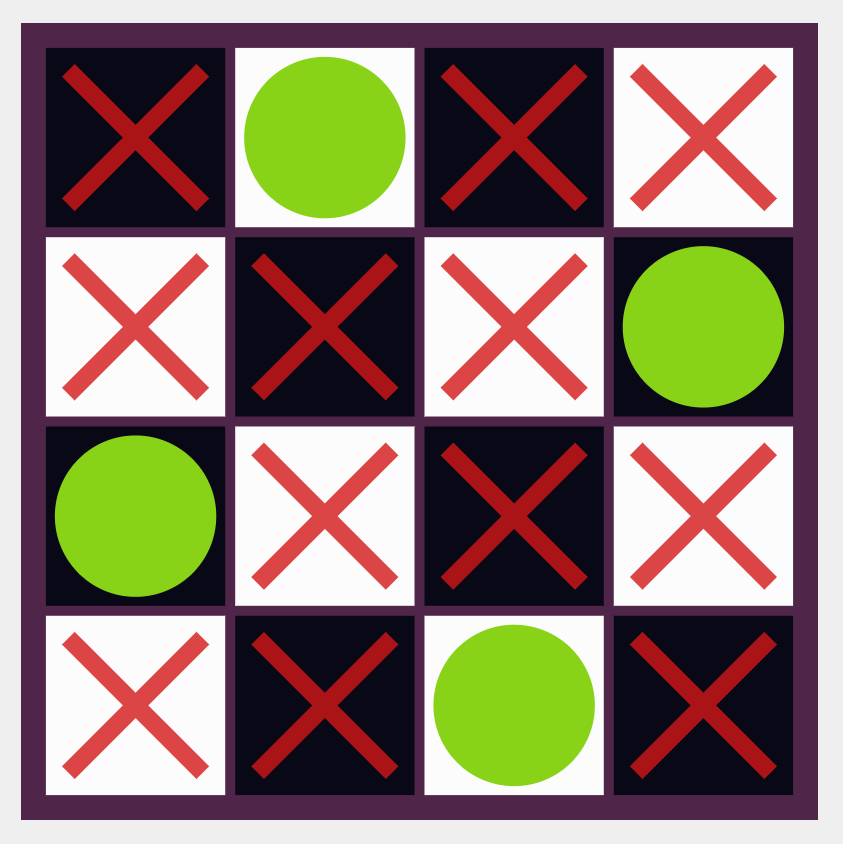
\includegraphics[width=0.7\textwidth]{img/Proof_Chessboard}
  \caption{Final Solution for 4-Queens Problem with Seed \enquote{Exmatrikulator}}
  \label{fig:design}
\end{figure}

Thus it is possible to replicate a certain result as often as possible and at any time. Thus the requirement is considered fulfilled.

\paragraph{Visualization of current progress}
The criterion here was to display the current solution process as a visual representation on the chessboard and as calculation steps. On the user interface, the animation is displayed visually in the middle of the chessboard and the calculations are shown in a box to the right. It should also be mentioned that this can either be done automatically or step by step with a single push of a button. The step size can also be adjusted. You can choose between Micro and Macro. Thus this requirement is also fulfilled.

\paragraph{Pausable Progress}
The requirement was that the simulation could be paused. If the user pressed the \enquote{Play} button, the simulation starts and at the same time the start button turns into a \enquote{Stop} button. This button can be used to stop the animation by pressing it. Please note, however, that the simulation only stops after the current calculation step has been completed. After this has been stopped, the button changes back to \enquote{Play} and the animation can be continued at the corresponding position.

\section{Conclusion}
\label{sec:proConclusion}
As shown in the previous section, this program meets all previously defined requirements. The program is considered successful and the project can now be completed satisfactorily. In summary, it was a very exciting project with no significant problems. Again and again during the implementation phase, the requirements had to be re-examined and decisions had to be made with the help of these decisions. The program had to be easy to use and understand at all times. Both usability and user experience played a role in all areas of the development process. 

The use of Javascript made web development a lot easier, but there were also some difficulties. But these were solved by helpful libraries and technologies like web workers. 

\section{Outlook}
\label{sec:proOutlook}
% cSpell:disable
%TODO Koen. Du musst sagen, wie man die Berechnung optimieren könnte
%Es gibt immer Bereiche eines Programms, die zukünftig noch verbessert werden können. Beispielsweise könnte die Berechnung der Lösung des N Damen Problems bestimmt noch weiter optimiert werden. Dadurch würde die Performanz eventuell verbessert werden, da vor allem bei großen Zahlen für N die Berechnung sehr lange dauert. 
%TODO Koen: durchlesen und eventuell ergänzen
%Eine weitere Idee zur zukünftigen Weiterentwicklung wäre die Verwendung dieses Programms für weitere aussagelogische Probleme und nicht nur das N Damen Problem. Durch die Verwendung der web worker wäre dies durch aus denkbar und umsetzbar. Somit ist der Davis Putman Algorithmus in diesem Programm universell einsetzbar.
%There are always areas of a program that can be improved in the future. For example, the calculation of the solution to the N-Queens Problem could certainly be further optimized. This would possibly improve the performance, because especially with large numbers for N the calculation takes a very long time. 
% cSpell:enable

There are always areas of a program that can be improved in the future for example the performance. But because the program is only used for small numbers of the N-Queens Problem, the speed of the calculations for the larger ones is not the focus for future improvements.  \\
\\
Another idea for future development would be the use of this program for further logical problems and not only the N-Queens Problem. By using the web worker this would be possible. Therefore the Davis Putman algorithm is universally applicable in this program.

% ------------------------------------------------------------------

\label{lastpage}

% Neue Seite
\cleardoublepage

% Backmatter mit normalem Zeilenabstand setzen
\singlespacing

% Römische Ziffern für die "Back-Matter", fortlaufend mit "Front-Matter"
\pagenumbering{roman}
\setcounter{page}{\value{frontmatterpage}}

% Abkürzungsverzeichnis
\addchap{\dhbwabbreviations}
\begin{acronym}
\acro{ABK}{Abkürzung}
\acro{ACM}{Association of Computing Machinery}
\acro{PDF}{Portable Document Format}
\acro{IEEE}{Institute of Electrical and Electronics Engineers}
\acro{ISO}{International Organization for Standardization}
%%%%%%%%%%%%%%%%%%%%%%%%%%%%%%%%%%%%%%%%%%%%%%%%%%%%%%%%%%%%%%%%
%a

%b

%c

%d

%e

%f

%g

%h

%i

%j

%k

%l

%m

%n

%o

%p

%q

%r

%s

%t

%u

%v

%w

%x

%y

%z

\end{acronym}



% Tabellenverzeichnis erzeugen
\cleardoublepage
\phantomsection
\addcontentsline{toc}{chapter}{\dhbwlistoftables}
\listoftables

% Abbildungsverzeichnis erzeugen
\cleardoublepage
\phantomsection
\addcontentsline{toc}{chapter}{\dhbwlistoffigures}
\listoffigures

%% Listingverzeichnis erzeugen
%\cleardoublepage
%\phantomsection
%\addcontentsline{toc}{chapter}{\dhbwlistings}
%\lstlistoflistings

% Literaturverzeichnis erzeugen
\begin{flushleft}
\printbibliography
\end{flushleft}

% Index ausgeben. Wenn Sie keinen Index haben, entfernen Sie einfach
% diesen Teil.
\cleardoublepage
\phantomsection
\addcontentsline{toc}{chapter}{\dhbwindex}
\printindex

% Anhang. Wenn Sie keinen Anhang haben, entfernen Sie einfach
% diesen Teil.
%\appendix
%\input{tex/anhang-a}
%\input{tex/anhang-b}

\end{document}





%\documentclass{report}
%\usepackage[utf8]{inputenc}
%\usepackage[english]{babel}
%\usepackage{graphicx}
%\usepackage{a4wide}
%%\usepackage{epsfig}
%
%\usepackage{hyperref}
%\usepackage[all]{hypcap}
%\hypersetup{
%	colorlinks = true,
%	linkcolor  = blue,
%	citecolor  = red,
%    filecolor  = gold,
%    urlcolor   = [rgb]{0.5, 0.0, 0.5},
%	pdfborder  = {0 0 0} 
%}
%
%\usepackage{fancyhdr}
%\usepackage{lastpage}
%
%\renewcommand*{\familydefault}{\sfdefault}
%
%\pagestyle{fancy}
%
%\fancyfoot[C]{--- \thepage/\pageref{LastPage}\ ---}
%
%\fancypagestyle{plain}{
%    \fancyhf{}
%    \fancyfoot[C]{--- \thepage/\pageref{LastPage}\ ---}
%    \renewcommand{\headrulewidth}{0pt}
%}
%
%\renewcommand{\chaptermark}[1]{\markboth{\chaptername \ \thechapter.\ #1}{}}
%\renewcommand{\sectionmark}[1]{\markright{\thesection. \ #1}{}}
%\fancyhead[R]{\leftmark}
%\fancyhead[L]{\rightmark}
%
%\author{Koen Loogman \& Jessica Roth}
%%\title{
\epsfig{file=dhbw-logo.eps, scale=1.0}\\[0.3cm]
%\title{ 
%        Animation N Queens Problem in Javascript\\[0.3cm]
%        DHBW Mannheim}
%\date{\today}
%

%
%
%\begin{document}
%
%    \maketitle
%    \tableofcontents
%
%    % !TeX root = ./documentation.tex

\chapter{Introduction}
\label{ch:introduction}

\section{Motivation}
\label{sec:introMotivation}
% cSpell:disable
%TODO Koen: Fällt dir was besseres ein?
%Der Davis Putman Algorithmus ist ein wichtiges Werkzeug zur Lösung von bekannten mathematischen Problemen wie beispielsweise das N Damen Problem. Dies ist auch der Grund, weshalb dieser oftmals zum Erklären von aussagelogischen Prinzipien verwendet wird. Oftmals ist es aber schwierig nachzuvollziehen, wie der ALgorithmus aussagelogische Probleme löst, da es allein durch das Betrachten der Rechenwege des Algorithmus nur schwer zu verstehen ist.
%\\
%Wenn es die Möglichkeit gäbe, die Lösung des N Damen Problems Schritt für Schritt zu verfolgen und dies visuell veständlich angezeigt zu bekommen, dann würde dies viele Verständnisprobleme klären und den Lernprozess deutlich beschleunigen. Dies ist auch der Grund, weshalb dieses Programm zur Visualisieren des Davis Putman Algorithmus so wichtig ist. Es kann zu vielen Zwecken wie beispielsweise der Unterstützung von Lehrveranstaltungen verwendet werden und hilft damit vielen Interessierten einen einfachen Einstieg in diesen komplexen Algorithmus.
% cSpell:enable
The \textit{Davis-Putman algorithm} is an important tool for solving known mathematical problems such as the \textit{N-Queens Problem}. This is also the reason why it is often used to explain propositional logic principles. However, it is often difficult to understand how the algorithm finds possible solutions for propositional logic problems, as it is difficult to understand by just looking at the algorithm's computational paths.

If there would be the possibility to follow the solution of the \textit{N-Queens Problem} step by step with a visual representation of the current state, then this would clarify many understanding problems and enhance the learning process. This is also the reason why this program is so important for visualizing the Davis Putman algorithm. It can be used for many purposes, such as supporting lectures, and thus helps many interested people to easily get started with this complex algorithm.

\section{Objective of the work}
\label{sec:introObjective}
% cSpell:disable
%TODO Koen: Fällt dir noch etwas dazu ein?
%Die Aufgabenstellung dieser Studienarbeit handelt von der Animation des Davis Putman Algorithmus anhand des N Damen Problems mit der Hilfe von Javascript. Dabei werden mehrere Kriterien definiert, die diese Animation erfüllen muss, da sie vor allem zur Visualisierung und zur genaueren anschaulichen Verdeutlichung beziehungsweise Erklärung des Algorithmus dient. Die genauen Anforderungen werden im Laufe dieser Arbeit genauer spezifiziert und am Ende am finalen Produkt evaluiert. Der Hauptteil dieser Arbeit handelt deshalb von der Konzeption und der Implementierung dieser Aufgabenstellung.
% cSpell:enable
The task of this student research project is the animation of the \textit{Davis-Putman algorithm} on the basis of the \textit{N-Queens Problem} with the help of JavaScript. Several criteria are defined, which this animation must fulfill, since it serves above all for the visualization and for the more exact descriptive clarification and/or explanation of the algorithm. The exact requirements are specified more precisely in the course of this work and evaluated at the end of the final product. The main part of this work therefore deals with the conception and implementation of this task.

\section{Structure of the report}
\label{sec:introStructure}
% cSpell:disable
%Um die Navigation durch diese Arbeit zu erleichtern, wird im folgenden Abschnitt einen kurzen Blick in die Struktur dieser Arbeit geworfen. 
%\\
%Im nächsten Kapitel werden die mathematischen Grundlagen zum Davis Putman Algorithmus und des N Damen Problems geschaffen. Dabei handelt es sich vor allem um die logischen Zusammenhänge und der mathematisch korrekten Definition des zu lösenden Problems. 
%\\
%Darauffolgend wird im dritten Kapitel ein allgemeiner Überblick zu den verwendeten Bibliotheken und Technologien gegeben und Hintergrundinformationen geliefert, aus welchen Gründen bestimmte Technologien bevorzugt beziehungsweise ausgewählt wurden.
%\\
%Im vierten Abschnitt dieser Arbeit wird die Konzeption des Programms genauer betrachtet. Vor allem handelt es von der allgemeinen Architektur und dem erstellten Layout Design, das als Vorlage für die Implementierung der Benutzeroberfläche dient. Eingeleitet wird das Kapitel durch das Spezifizieren der Anforderungen für das Programm, die eine zentrale Rolle in der Evaluation am Ende spielen.
%\\
%Im fünften Kapitel wird nun Schritt für Schritt durch die fertige Implementierung geleitet und der Aufbau des Programms genauer erläutert. Dabei wird durch die unterschiedlichen Komponenten und Klassen geführt und dabei ihre Funktion genauer erläuert.
%\\
%Das letzte Kapitel wird mit der Evaluation der Anforderungen begonnen. Dies dient vor allem dazu, um zu schauen, ob das Programm alle Kriterien erfüllt und zu Ende als erfolgreich erfüllt angesehen werden kann. Danach folgt ein zusammenfassendes Fazit und ein Ausblick, wie das Programm zukünftig weiterentwickelt oder anders eingesetzt werden könnte.
% cSpell:enable
In order to facilitate navigation through this work, the following section takes a brief look at the structure of this work.

In the next chapter explains the scientific basics of the \textit{Davis-Putman algorithm} and the \textit{N-Queens Problem}. These are mainly about the logical correlations and the mathematically correct definition of the problem to be solved.

The third chapter then gives a general overview of the libraries and technologies used and provides background information on the reasons why certain technologies were preferred or selected.

The fourth section of this paper takes a closer look at the design of the program. It mainly deals with the general architecture and the created layout design, which serves as a template for the implementation of the user interface. The chapter is introduced by specifying the requirements for the program, which are mandatory for the evaluation at the end.

In the fifth chapter, step by step you will be guided through the finished implementation and the structure of the program will be explained in more detail. The different components and classes are guided through and their roles explained in more detail.

The last chapter starts with the evaluation of the requirements. This is mainly to see if the program meets all the criteria and can be considered successful at the end. This is followed by a summary and an outlook on how the program or its components could be further developed or used in other ways in the future.
%    % !TeX root = ../documentation.tex

% Davis Putnam in own word

\chapter{Scientific Basics}
\label{ch:sciBasics}
% cSpell:disable
% Das Ziel dieser Arbeit besteht in der Visualisierung des \textit{Davis-Putman algorithm}us, der das sogenannte N damen Problem lösen soll. Dafür muss zuerst ein allgemeines Verständnis zu diesem Algorithmus und dem mathematischen Problem geschaffen werden. In diesem Kapitel wird aus diesem Grund dieses fundamentale Wissen zusammengefasst, um eine Basis für die weiterführende Entwicklung zu schaffen. Dafür spielt unter anderem die Deklarierung des mathematischen Problems eine Rolle, damit dieses vom \textit{Davis-Putman algorithm}us gelöst werden kann.
% cSpell:enable
The purpose of this work is to visualize the \textit{Davis-Putnam algorithm} solving the so-called \textit{N-Queens Problem}. Therefore a general understanding of this algorithm and the mathematical problem has to be created.

This chapter summarizes the fundamental knowledge that is needed in order to create a basis for further development. Among other things, the definition of the mathematical problem plays a role here, so that a possible solution can be found by the \textit{Davis-Putnam algorithm}.

\section{Basics of Propositional Logic}
\label{sec:sciProLogic}
Before the algorithm can be examined in more detail, a few mathematical terms must first be briefly explained.

\paragraph{Propositional logic interpretation}
The function $\mathcal{I}:\mathcal{P} \rightarrow \mathbb{B}$ is called propositional logic interpretation, which assigns a true value $\mathcal{I}(p) \in \mathbb{B}$ to each proposition-logical variable $p\in \mathcal{P}$

\paragraph{Satisfiable}
There is a set of propositional logic formulas. If there is an interpretation $I$ so that all formulas are satisfied and the formula $\mathcal{I}(f) = \texttt{True}$ \quad for all propositional logic formulas in the set is given, so this set is satisfiable. If this is not the case, then this set is not satisfiable.

\paragraph{Tautology}
A propositional logic formula $f$ is a tautology if and only if $\mathcal{I}(f) = \texttt{True}$ for every interpretation $\mathcal{I}$. In this case it is written as $\models f$.

\paragraph{Literal}
A propositional logic formula $f$ is called a literal, if one of the following cases is true.

\begin{enumerate}
  \item $f = \top$ or $f = \bot$
  \item $f = p$, where $p$ is a propositional variable. If this is the case, it is called a positive literal.
  \item $f = \neg p$, where $p$ is a propositional variable. Then it is called a negative literal.
\end{enumerate}

\paragraph{Clause}
A propositional logic formula $C$ is called a clause if it has the following structure.
\\[0.2cm]
\hspace*{1.3cm} $C = l_1 \vee \cdots \vee l_r$ \\[0.2cm] Here, $l_i$ is a literal for every value $i \in \{1,\; ...,\; r\}$.

\section{The Algorithm of Davis-Putnam}
\label{sec:sciDavisPutnam}
% cSpell:disable
% Der \textit{Davis-Putman algorithm}us ist ein Verfahren zur Berechnung einer Lösung von aussagelogischen Klauselmengen. Bei sehr kleinen Klauselmengen kann dies leicht bestimmt werden, wie in den zwei folgenden Beispielen zu sehen ist.
% cSpell:enable
The \textit{Davis-Putnam algorithm} is a method for calculating a solution of a set of propositional clauses. With clause sets that contain just one literal per clause this can be easily determined, as can be seen in the following two examples.
\\[0.2cm]
\hspace*{1.3cm} $K_1 = \bigl\{\; \{r\},\; \{\neg s\},\; \{t\},\; \{\neg u\}, \; \{\neg v\} \;\bigr\}$ 
\\[0.2cm]
% cSpell:disable
%kann auch als aussagelogische Formel geschrieben werden.
% cSpell:enable
$K_1$ can also be written as a propositional logic formula.
\\[0.2cm]
\hspace*{1.3cm} $r \land \neg s \land t \land \neg u \land \neg v$.
\\[0.2cm]
% cSpell:disable
% Es ist erkennbar, dass diese Formel lösbar ist, indem $r$ und $t$ \enquote{wahr} und $s$, $u$ und $v$ den Wert \enquote{falsch} haben. Als Gegenbeispiel dazu ist $K_2$ zu betrachten.
% cSpell:enable
It is obvious that this formula is solvable by $r$ and $t$ \enquote{true} and $s$, $u$ and $v$ having the value \enquote{false}.
As a negative example we consider the set $K_2$, which is defined as follows:
\\[0.2cm]
\hspace*{1.3cm} $K_2 = \bigl\{\; \{r\},\; \{\},\; \{t\} \;\bigr\}$
\\[0.2cm]
$K_2$ can also be written as a propositional logic formula.
\\[0.2cm]
\hspace*{1.3cm}
$r \land \bot \land t$.
\\[0.2cm]
% cSpell:disable
% Eine leere Klammer bedeutet in der Aussagelogik ein Falsum, wodurch $K_2$ unerfüllbar ist. Bei sehr großen Klauselmengen ist es meist nicht mehr auf dem ersten Blick zu sehen, so dass Algorithmen wie dieser eingesetzt werden. Doch um nun einen Schritt tiefer setzen zu können, müssen zwei Definitionen zuvor eingeführt werden.
% cSpell:enable
The empty set in the set of clauses $K_2$ is interpreted as a $\bot$ in the propositional logic, making it impossible to satisfy $K_2$. It is possible to satisfy smaller sets of less complex clauses by first glance, but it gets more difficult for larger and more complex sets of clauses. For these algorithms like the \textit{Davis-Putnam algorithm} are used. But before we get to the details, two definitions have to be introduced first \cite{Zhang2000}. 

\paragraph{Unit clause}
% cSpell:disable
% Eine Klausel $C$ ist eine Unit-Klausel, wenn diese nur aus einem Literal, also aus einer Aussagevariablen besteht.
% cSpell:enable
A clause $C$ is a unit clause if it contains of only a single literal, i.e. a variable or a negated variable.

\paragraph{Trivial clause sets}
% cSpell:disable
% Eine triviale Klauselmenge kann nur vorkommen, wenn einer der beiden Fälle eintritt.
% cSpell:enable
A set of clauses is trivial if and only if one of the following two cases occurs.

\begin{enumerate}
  % cSpell:disable
  % $K$ enthält die leere Klausel und ist somit unerfüllbar
  % cSpell:enable
  \item A set of clauses $K$ contains the empty set and is therefore unsatisfiable.
  % cSpell:disable
  % Die Unit-Klauseln beinhalten immer verschiedene Aussagevariablen, so dass entweder nur die Klausel $\{p\}$ oder $\{\neg p\}$ vorkommen kann. Ist dies der Fall, kann eine Lösung für die Klauselmenge bestimmt werden.
  % cSpell:enable
  \item The unit clauses always contain different propositional variables, so that only the clause $\{p\}$ or $\{\neg p\}$ can occur. If this is the case, a solution for the clause set can be determined.
\end{enumerate}

% cSpell:disable
% Damit einer dieser beiden Fälle nun eintreten kann, müssen die Klauselmengen mit der Hilfe folgender drei Möglichkeiten so vereinfacht werden, dass diese nur aus Unit-Klauseln bestehen.
% cSpell:enable
In order for one of these two cases to occur, the clause sets must be simplified with the help of the following three options so that they consist only of unit clauses.

\begin{enumerate}
  \item Cut Rule 
  \item Subsumption
  \item Case Differentiation
\end{enumerate}

\subsection{Simplification with the Cut Rule}
\label{sub:sciDavisPutnamCutRule}
To simplify a set of clauses $K$ with $C_1 \cup \{\; p\; \}$, $C_2 \cup \{\; \neg p\; \} \in K$ the cut rule can be used. Let's say we have two clauses $C_1$, $C_2$ and a variable $p$, then a typical application of the cut rule is.
\\[0.2cm]
\hspace*{1.3cm} $\dfrac{C_1 \cup \{\; p\; \} \;\;\;\;\;\; C_2 \cup \{\; \neg p\; \}}{C_1 \cup C_2}$
\\[0.2cm]
In this case the result clause will in general have more literals than $C_1 \cup \{\; p\; \}$ or $C_2 \cup \{\; \neg p\; \}$ alone. Because if the clause $C_1 \cup \{\; p\; \}$ contains $m + 1$ literals and $C_1 \cup \{\; p\; \}$ contains $n + 1$ literals, then the union $C_1 \cup C_2$ can have upto $m + n$ literals in total. In general $m + n$ may be bigger than $m + 1$ or $n + 1$. The clause can be smaller than previously if both sets contain the same literals, but it is only granted to be smaller if $m = 0 \lor n = 0$. This is the case for unit clauses. Therefore we will only allow the use of the cut rule if one of the clauses is a unit clause. These cuts will be called unit cuts. To be able to do those unit cuts with a unit clause $\{\; l\; \}$ on all clauses of a set of clauses $K$, we define the function
\\[0.2cm]
\hspace*{1.3cm} $\texttt{unitCut}: 2^{K} \times L \to 2^{K}$
\\[0.2cm]
so that for a set of clauses $K$ and a literal $l$ the function $\texttt{unitCut}(K,\; l)$ will simplify the set of clauses as much as possible by using unit cuts:
\\[0.2cm]
\hspace*{1.3cm} $\texttt{unitCut}(K,\; l) = \{\; C \setminus \{\; \bar{l}\; \}\; |\; C \in K\; \}$
\\[0.2cm]
The result set of clauses will have the same amount of clauses as $K$. Only the clauses $C \in K$ where $\bar{l} \in C$ were affected and got that element removed \cite{Stroetman2019}. 

\subsection{Simplification with Subsumption}
\label{sub:sciDavisPutnamSubsumption}
For further simplification of the set of clauses we will use subsumption. The idea is simple and can be shown with the following example:
\\[0.2cm]
\hspace*{1.3cm} $K = \{\; \{\; p,\; \neg q \;\},\; \{\; p\; \}\; \} \cup M$
\\[0.2cm]
It is clear that the clause $\{\; p\; \}$ implies the clause $\{\; p,\; \neg q \;\}$, because if $\{\; p\; \}$ is satisfied, then $\{\; p,\; \neg q \;\}$ will be satisfied too. That's because
\\[0.2cm]
\hspace*{1.3cm} $\models p \to p \lor \neg q$
\\[0.2cm]
is given. With that in mind we can say that we can subsume a clause $C$ with a unit clause $U$ if $U \subseteq C$. That means if we have a set of clauses $K$ with $C \in K \land U \in K$ and $U$ subsumes $C$, we can remove the clause $C$ from $K$ to reduce its size. We define a function
\\[0.2cm]
\hspace*{1.3cm} $\texttt{subsume}: 2^{K} \times L \to 2^{K}$
\\[0.2cm]
that receives a set of clauses $K$ and a literal $l$. It will simplify $K$ by subsuming with the unit clause $\{\; l\; \}$:
\\[0.2cm]
\hspace*{1.3cm} $\texttt{subsume}(K,\; l) = \{\; C \in K\; |\; l \notin C\} \cup \{\{\; l\; \}\}$
\\[0.2cm]
We have to add the unit clause to the set of clauses, because $l \in U$ is the case. Resulting in $U$ being removed from $K$ at first too \cite{Stroetman2019}. 

\subsection{Simplification with Case Differentiation}
\label{sub:sciDavisPutnamCaseDiv}
% cSpell:disable
% Die Basis für das Prinzip der Fallunterscheidung bildet folgender Satz.
% cSpell:enable
The following theorem forms the basis for the principle of case differentiation.

\paragraph{Theorem}
% cSpell:disable
% Die Klauselmenge K ist genau dann erfüllbar, wenn die Klausel $K \cup \bigl\{\{p\}\bigr\}$ oder $K \cup \bigl\{\{\neg p\}\bigr\}$ erfüllbar ist.
% cSpell:enable
The set of clauses $K$ can only be satisfied if and only if $K \cup \bigl\{\{p\}\bigr\}$ or $K \cup \bigl\{\{\neg p\}\bigr\}$ can be satisfied.

% cSpell:disable
% Für die Vereinfachung wird zu Beginn also eine Aussagenvariable p ausgewählt, die in der Klauselmenge vorkommt. Danach werden die beiden oben genannten Klauselmengen gebildet und versucht, für eine der beiden eine Lösung zu finden. Ist dieser Versuch erfolgreich, ist das Ergebnis automatisch die Lösung von $K$. Falls keine gefunden wird, ist $K$ unlösbar.
% TODO: Keine Ahnung ob hier Beweis einfügen soll
% cSpell:enable
For simplification, a propositional variable $p$ is selected at the beginning, which occurs in the clause set. Then the two clause sets mentioned above are formed and an attempt is made to find a solution for one of them. If this attempt is successful, the result is automatically a solution of $K$. If none is found, $K$ is not satisfiable.

\subsection{The Davis-Putnam Method}
\label{sub:sciDavisPutnamMethod}
% cSpell:disable
% Durch die Wissensgrundlage, die zuvor geschaffen wurde, ist es nun möglich, das Vorgehen des \textit{Davis-Putman algorithm}us zu skizzieren. Mit der Hilfe der Schnittregel und der Subsumption wird die Klauselmenge $K$ soweit es möglich ist, vereinfacht. Falls bereits nach diesem Schritt $K$ trivial ist, ist das Verfahren beendet. Andernfalls wird eine aussagelogische Variable p ausgewählt, die in K vorkommt. Dann wird rekursiv versucht, die Klauselmenge $K \cup \bigl\{\{p\}\bigr\}$ zu lösen, um eine Lösung für K zu finden. Wenn auch hier keine Lösung gefunden wurde, wird dasselbe mit dem negierten $p$ versucht. Scheitert auch dieser Versuch, ist K unlösbar.
% cSpell:enable
The theoretical foundation that was previously created now makes it possible to sketch the procedure of the \textit{Davis-Putnam algorithm}. With the help of the intersection rule and the subsumption, the clause set $K$ is simplified as far as possible. If already after this step $K$ is trivial, the procedure is finished. Otherwise a propositional logical variable p is selected, which occurs in $K$. Then a recursive attempt is made to solve the clause set $K \cup \bigl\{\{p\}\bigr\}$ in order to find a solution for $K$. If no solution was found here either, the same is tried with the negated $p$. If this attempt also fails, $K$ is unsatisfiable. A possible recursive implementation of the method can be seen in listing \ref{code:recursiveDavisPutnam} \cite{Zhang2000}, \cite{Stroetman2019}.
% TODO: find more sources

\begin{listing}[h!]
  \textbf{function} Satisfiable( clause set $S$ ) \textbf{return} boolean\\
    \hspace*{0.5cm} \textit{/* unit propagation */}\\
    \hspace*{0.5cm} \textbf{repeat}\\
      \hspace*{1.0cm} \textbf{for each} unit clause $L$ in $S$ \textbf{do}\\
        \hspace*{1.5cm} \textit{/* unit subsumption */}\\
        \hspace*{1.5cm} delete from $S$ every clause containing $L$\\
        \hspace*{1.5cm} \textit{/* unit resolution */}\\
        \hspace*{1.5cm} delete $\bar{L}$ from every clause of $S$ in which it occurs\\
      \hspace*{1.0cm} \textbf{od}\\
      \hspace*{1.0cm} \textbf{if} $S$ is empty \textbf{then}\\
        \hspace*{1.5cm} \textbf{return} true\\
      \hspace*{1.0cm} \textbf{else if} a clause becomes $\{\}$ in $S$ \textbf{then}\\
        \hspace*{1.5cm} \textbf{return} false\\
      \hspace*{1.0cm} \textbf{fi}\\
    \hspace*{0.5cm} \textbf{until} no further changes result\\
    \hspace*{0.5cm} \textit{/* splitting */}\\
    \hspace*{0.5cm} choose a literal $L$ occurring in $S$\\
    \hspace*{0.5cm} \textbf{if} Satisfiable ($S \cup \{\{\bar{L}\}\}$) \textbf{then}\\
      \hspace*{1.0cm} \textbf{return} true\\
    \hspace*{0.5cm} \textbf{else if} Satisfiable ($S \cup \{\{L\}\}$) \textbf{then}\\
      \hspace*{1.0cm} \textbf{return} true\\
    \hspace*{0.5cm} \textbf{else}\\
      \hspace*{1.0cm} \textbf{return} false\\
    \hspace*{0.5cm} \textbf{fi}\\
  \textbf{end function}
  \caption{A simple Davis–Putnam algorithm \cite{Zhang2000}}
  \label{code:recursiveDavisPutnam}
\end{listing}

\section{N-Queens Problem}
\label{sec:sciQueens}
% cSpell:disable
% Das n Königinnen Problem ist das verallgemeinerte mathematische Problem bezogen auf ein Schachbrett, dass n \times n Felder besitzt. Ein spezielles Beispiel dazu wäre das 8 Damen Problem, welches auf dem standardisierten Schachbrett abgebildet wird. Allgemein handelt das Problem davon, n Damen auf einem n \times n Schachbrett so zu platzieren, dass keine in ihrem Zug behindert werden würde. Eine Königin in einem normalen Schachspiel kann sowohl diagonal, als auch vertikal und horizontal ihre Züge ziehen. Dieses Zugmuster kann in Figure \label{fig:queens-problem} genauer angeschaut werden. Zusammengefasst heißt dies also, dass immer nur eine Dame auf ihrer vertikalen, horizontalen und diagonalen Linie sein darf, um sich nicht gegenseitig zu behindern. Dabei wird in diesem Problem davon ausgegangen, dass jede Dame jede andere angreifen kann und die Feldfarben ignoriert werden. 
% cSpell:enable
The N-Queens Problem is the generalized mathematical problem related to a chessboard that consists of $n \times n$ squares. A special example would be the 8-Queens Problem, which is related to the standardized chessboard. In general, the problem is to place n queens on an $n \times n$ chessboard so that none would be obstructed in their turn. A queen in a normal game of chess can move diagonally, vertically and horizontally. This move pattern can be seen in Figure \ref{fig:queens-problem}. In summary, this means that there is only one queen allowed on her vertical, horizontal and diagonal line at a time so that they do not interfere with each other. In this problem it is assumed that any queen can attack any other queen and the field colors are ignored. This problem can be solved by several algorithms such as the \textit{Davis-Putnam algorithm} \cite{Bell2009}, \cite{Watkins2012}, \cite[146\psq]{Nudelman1995}, \cite{Stroetman2019}.

\begin{figure}[!ht]
  \centering
  \setlength{\unitlength}{1.0cm}
  \begin{picture}(10,9)
    \thicklines
    \put(1,1){\line(1,0){8}}
    \put(1,1){\line(0,1){8}}
    \put(1,9){\line(1,0){8}}
    \put(9,1){\line(0,1){8}}
    \put(0.9,0.9){\line(1,0){8.2}}
    \put(0.9,9.1){\line(1,0){8.2}}
    \put(0.9,0.9){\line(0,1){8.2}}
    \put(9.1,0.9){\line(0,1){8.2}}
    \thinlines
    \multiput(1,2)(0,1){7}{\line(1,0){8}}
    \multiput(2,1)(1,0){7}{\line(0,1){8}}
    \put(4.15,6.15){{\chess Q}}
    \multiput(5.25,6.5)(1,0){4}{\vector(1,0){0.5}}
    \multiput(3.75,6.5)(-1,0){3}{\vector(-1,0){0.5}}
    \multiput(5.25,7.25)(1,1){2}{\vector(1,1){0.5}}
    \multiput(5.25,5.75)(1,-1){4}{\vector(1,-1){0.5}}
    \multiput(3.75,5.75)(-1,-1){3}{\vector(-1,-1){0.5}}
    \multiput(3.75,7.25)(-1,1){2}{\vector(-1,1){0.5}}
    \multiput(4.5,7.25)(0,1){2}{\vector(0,1){0.5}}
    \multiput(4.5,5.75)(0,-1){5}{\vector(0,-1){0.5}}
  \end{picture}
  \vspace*{-1.0cm}
  \caption{Movement pattern of a queen on an 8 by 8 board \cite{Stroetman2019}} 
  \label{fig:queens-problem}
\end{figure}

\subsection{N-Queens Problem as Propositional Formula}
Before we can find a solution for the \textit{N-Queens Problem}, we need to define the problem as a propositional logic formula. For that we will say that the variable $Q_{x,y}$ is the queen in row $x$ on column $y$. If said variable is true a queen will be placed and if not a queen can not be placed. Now all that is left is the creation of the set of clauses $K$ that describes the \textit{N-Queens Problem}. Therefore we create some functions to help us define the problem as such:

\paragraph{atMostOne}
The function atMostOne will receive a set of literals $L$ and return a set of clauses $K$ that express the fact that only one of the literals $l \in L$ can be true. We define it to support following functions.
\\[0.2cm]
\hspace*{1.3cm}$\texttt{atMostOne}:\ \mathcal{L} \to 2^{\mathcal{K}}$
\\[0.2cm]
\hspace*{1.3cm}$\texttt{atMostOne}(L) := \{\ \{\ \neg l_1,\ \neg l_2 \}\ :\ l_1, l_2 \in L\ |\ l_1 \neq l_2\ \}$
\\[0.2cm]
This works, because if one variable is said to be true then the other variable must be false, since either one or the other needs to be false.

\paragraph{atMostOneInRow}
This function receives a number $n$ for the total amount of queens and a number $r \in \{1 .. n\}$ for the row and return a set of clauses $K$ that express the fact that only one queen can be placed in row $r$.
\\[0.2cm]
\hspace*{1.3cm} $\texttt{atMostOneInRow}:\ \mathcal{N} \times \mathcal{N} \to 2^{\mathcal{K}}$
\\[0.2cm]
\hspace*{1.3cm} $\texttt{atMostOneInRow}(r,\ n) := \texttt{atMostOne}(\{\ Q_{r,i} :\ i \in \{1\ ..\ n\}\ \})$

\paragraph{oneInColumn}
This function receives a number $n$ for the total amount of queens and a number $c$ where $c \leq n$ for the column and returns a set of clauses $K$ that express the fact that at least one queen has to be placed in the column $c$. Because if only one queen can be placed per row, every column needs at least one queen to have $n$ queens on the chessboard.
\\[0.2cm]
\hspace*{1.3cm} $\texttt{oneInColumn}:\ \mathcal{N} \times \mathcal{N} \to 2^{\mathcal{K}}$
\\[0.2cm]
\hspace*{1.3cm} $\texttt{oneInColumn}(c,\ n) := \{\ \{\ Q_{i,c} :\ i \in \{1\ ..\ n\}\ \}\ \}$

\paragraph{atMostOneInUpperDiagonal}
This function returns a set of clauses $K$ that express the fact that only one queen can be placed in the upper diagonal, for a given number $n$ and $k \in \{3\ ..\ 2 * n - 1\}$. The number $k$ helps with calculating which combination of row and column is part of the diagonal.
\\[0.2cm]
\hspace*{1.3cm} $\texttt{atMostOneInUpperDiagonal}:\ \mathcal{N} \times \mathcal{N} \to 2^{\mathcal{K}}$
\\[0.2cm]
\hspace*{1.3cm} $\texttt{atMostOneInUpperDiagonal}(k,\ n) :=$
\hspace*{2.6cm} $\texttt{atMostOne}(\{\ Q_{x,y} :\ x,y \in \{1\ ..\ n\}\ |\ x + y = k\ \})$

\paragraph{atMostOneInLowerDiagonal}
This function returns a set of clauses $K$ that express the fact that only one queen can be placed in the lower diagonal, for a given number $n$ and $k \in \{-(n - 2)\ ..\ n - 2\}$. As before the number $k$ helps with calculating which combination of row and column is part of the diagonal.
\\[0.2cm]
\hspace*{1.3cm} $\texttt{atMostOneInLowerDiagonal}:\ \mathcal{N} \times \mathcal{N} \to 2^{\mathcal{K}}$
\\[0.2cm]
\hspace*{1.3cm} $\texttt{atMostOneInLowerDiagonal}(k,\ n) := \texttt{atMostOne}(\{\ Q_{x,y} :\ x,y \in \{1\ ..\ n\}\ |$
\hspace*{11.5cm} $\ x - y = k\ \})$

\paragraph{queensClauses}
With the functions above, we finally can define the complete propositional formula for the \textit{N-Queens Problem} for a given number $n$ in form of a set of clauses $K$. Here a set of clauses that express that only one queen can be placed per column is not needed, because that one has to be placed in combination with only one per row implies that only one per column is placed.
\\[0.2cm]
\hspace*{1.3cm} $\texttt{queensClauses}: \mathcal{N} \to 2^{\mathcal{K}}$
\\[0.2cm]
\hspace*{1.3cm} $\texttt{queensClauses}(n) := \bigcup\limits_{i=1}^{n}(\texttt{atMostOneInRow}(i, n)\ \cup\ $
%\\[0.1cm]
%\hspace*{6.5cm}
$\texttt{oneInColumn}(i, n))\ \cup\ $
\\[0.1cm]
\hspace*{6.1cm} $\bigcup\limits_{i=3}^{2 * n - 1}\ \texttt{atMostOneInUpperDiagonal}(i, n)\ \cup\ $
\\[0.1cm]
\hspace*{5.8cm} $\bigcup\limits_{i=-(n - 2)}^{n - 2}\texttt{atMostOneInLowerDiagonal}(i, n)$
%    % !TeX root = ./documentation.tex

% Javascript und verwendete Libraries

\chapter{Technical Basics}
Im vorherigen Kapitel wurden die Grundlagen zum Davis Putman Algorithmus und des N Damen Problems genauer analysiert und definiert. Nun folgt eine Sammlung von Bibliotheken und Technologien, die für die Implementierung benötigt werden. Dabei wird vor allem auf den Einsatz dieser und der Vergleich zu eventuellen Alternativen eingegangen. 

\section{Parcel}
%TODO Koen: Sollten wir Module Bundling noch im Allgemeinen erklären oder weglassen oder ins Implementierungs Kapitel schieben?
%TODO Jessica: Ansich eine grobe Erklärung wäre gut. Es ist ja ein Node.js feature. Plain JS hat keine dependencies oder modules. Es erhöt die Wartbarkeit und gestalltet die Entwicklung für OO-Programmierung einfacher.
Parcel ist ein Module Bundling Tool zur Integration von mehreren Modulen in eine Datei. Dadurch ist es möglich, multiple Module in einem einzigen Bundle an den Browser zu senden. Diese Bibliothek bietet einige sehr nützliche Funktionen an, die die Implementierung deutlich vereinfachen. Parcel nutzt Worker Prozesse, um eine multicore Compilierung zu ermöglichen und besitzt ein Filesystem Cache, um sehr schnelles Rebuilden zu ermöglichen. Dadurch ist Parcel vor allem auf Performanz im Browser ausgelegt. Um diese zusätzlich zu erhöhen, teilt Parcel die Output Bundles auf, so dass nur die benötigten Teile beim initialen Start geladen werden. Außerdem besitzt diese Bibliothek einen automatischen Support für Sprachen wie beispielsweise Javascript und CSS, wodurch keine Plugins benötigt werden. Der Programmcode und auch die Nodejs Module werden außerdem automatisch transformiert. Das ist sehr wichtig für dieses Projekt, da mit Nodejs und Pack dependencies gearbeitet wird. Ein weiteres interessantes Feature von Parcel ist das automatische Updaten der Module im Browser, wenn Änderungen durch die Entwicklung angewendet werden müssen. Das macht den Arbeitsprozess dynamisch und schneller. Das übersichtliche und verständliche Error Logging erleichtert zusätzlich dazu die Implementierung. 
%TODO Quellen einbauen (\url{https://parceljs.org/}). 
\subsection{Aktuelle Alternativen}
Parcel ist natürlich nicht das einzige Module Bundling Tool, sondern es gibt viele ähnliche Tools. Die zwei bekannten Tools Webpack und Rollup werden im folgenden Abschnitt grob angerissen und im kurzen Vergleich zu Parcel gestellt.
\paragraph{Webpack} Webpack wurde dazu erschaffen, Probleme mit dem Asset Management sinnvoll zu lösen und die Entwickler darin zu unterstützen. Dies ist auch der Grund, weshalb auch nicht-javascript Dateien eingebunden werden können. Während Parcel Out-of-the-box Support für viele Sprachen bereits mitbringt, kann Webpack durch eine Vielzahl an Plugins den Gegebenheiten angepasst und erweitert werden. Im Gegensatz zu Parcel benötigt Webpack eine config file, um die Optionen zu entry, output, plugin etc. genauer spezifieren zu können. Parcel benötigt keine und funktioniert automatisiert. Ein weiterer Unterschied ist, dass Webpack grundsätzlich eine Javascript Datei als entry point benötigt und nicht wie Parcel auch einen HTML Einstiegspunkt unterstützt. Dies kann zwar durch Drittanbieter Plugins gewährleistet werden, wird aber nicht automatisch mitgeliefert. Um einen Bundler zu erschaffen, müssen alle Formate in Javascript umgewandelt werden. Dies wird Transformation genannt. Während Webpack Loaders nutzt, die im Config File definiert werden müssen, unterstützt Parcel viele Formate ohne einen zusätzlichen Aufwand des Entwicklers. Unter gewissen Voraussetungen kann Webpack auch die Tree Shaking Funktion unterstützen, die für die dead code Eliminierung zuständig ist. Das wäre unter anderem das Nutzen des Format  ES2015, einen "sideEffect" entry im package.json File und das Hinzufügen eines minifers, der dead code Entfernung unterstützt. Parcel unterstützt diese Funktion in keiner Weise. Um einen Entwicklungsserver aufzubauen, der die Entwicklung und das Testen von Programmen erleichtert, muss in Webpack ein Plugin und die entsprechenden Konfigurationen hinzugefügt werden. Parcel hat einen eingebauten Entwicklungsserver, der bei jeder Änderung automatisch die Dateien neu aufbaut. Webpack unterstützt genauso wie Parcel das Hot Module Replacement. Code Splitting, um nur die benötigten Ressourcen zu Beginn zu laden und somit die Performanz im Browser zu verbessern, ist ein sehr ausgeprägtes Feature in Webpack. Dieses bietet drei Ansätze zur Umsetzung an, zwischen denen der Nutzer wählen kann. Einmal kann der Code anhand der entry Konfiguration manuell gesplittet werden, dann kann mit der Hilfe eines Plugins chunks geteilt werden und die letzte Möglichkeit ist die Aufteilung mithilfe von Inline Function Calls. Parcel unterstützt nur einen Ansatz zum Code Splitting: zero configuration code splitting. Hier wird die AUfteilung durch die dynamische import Function kontrolliert, wodurch die Module asynchron geladen werden.
\\
Trotz der großen Vielzahl der Möglichkeiten, die Webpack durch die Plugins erhält, wurde gegen dieses Tool entschieden, da deutlich mehr Zeit in die Konfiguration investiert werden müsste, währenddessen Parcel keine benötigt. Parcel beinhaltet die benötigten Features schon und ist sofort startbereit, welches den schnellen Entwicklungsprozess noch weiter antreibt. Dadurch ist es einfacher und effizienter, Parcel für die Entwicklung zu nutzen, da kein großes Vorwissen benötigt wird und durch die konfigurationsarme Verwendung einfacher zu nutzen ist.

\paragraph{Rollup}Rollup ist ein Module Bundler für Javascript, welcher kleine Codesnippets in ein großes Gesamtbild zusammenfügt. Dafür wird das neue standarisierte Format ES2015 für Code Modules verwendet. Wie auch Webpack benötigt Rollup eine Config Datei, während Rollup aber auch relative Pfade und node polyfills unterstützt. Dafür muss vor der Entwicklung Zeit investiert werden, während in parcel bereits ohne Konfiguration gestartet werden kann. Um die gleiche Funktionalität von Parcel zu bieten, dass HTML auch als Entry point verwendet werden kann, muss ein Plugin für Rollup installiert werden. Während Parcel die Transformation für die Bundleerstellung automatisch durchführt, muss für Rollup ein passendes Plugin gewählt und in der config file spezifiziert werden.  Rollup unterstützt Tree Shaking ohne jegliche Voraussetzungen im Gegensatz zu Webpack. Dabei überprüft Rollup den zu importierenden Coden und exclude die aktuell nicht verwendeten Funktionen. Parcel unterstützt diese Funktion wie bereits oben genannt leider nicht. Um einen Entwicklungsserver zu nutzen, muss auch hier ein zusätzliches Plugin installiert und konfiguriert werden. Um eine Live reload Funktion zu haben, muss sogar noch ein weiteres Plugin hinzugefügt und eingerichtet werden. Es ist deutlich zeitaufwändiger als die Hands-on Unterstützung bei Parcel zu nutzen. Leider unterstützt Rollup nicht wie Parcel oder Webpack die Hot Module Replacement und verbessert somit nicht die Performanz im Browser. Im Bereich des Code Splitting gibt es bisher nur experienteller Code, der chucks in standadisierte ES module spaltet, die dann vom module loader aufgerufen werden. Dafür müssen aktuell zwei Flags in der Config File anders gesetzt werden.
\\
Auch nach diesem Vergleich ist die Entscheidung auf Parcel gefallen, da Rollup wichtige Features fehlen, die relevant für das Projekt sind und auch hier wie bei Webpack der Konfigurationsaufwand deutlich höher ist wie bei Parcel.
%TODO Quellen einbauen https://medium.com/js-imaginea/comparing-bundlers-webpack-rollup-parcel-f8f5dc609cfd
%https://webpack.js.org/concepts
%https://rollupjs.org/guide/en

\section{Immutablejs}
In der späteren Umsetzung des Davis Putman Algorithmus wird ein bekanntes Problem bei der Benutzung mit Javascript auftauchen. Es handelt sich dabei um das Vergleichen zwischen Sets. Das native Set vergleicht Objekte dabei über die Object by Object Reference. Vergleiche mit mutable Objekten ist meist sehr schwierig, da wenn ein Objekt sich ändert, sich die Lokation dieser in einer Collection auch ändert. Die Bibliothek Immutablejs ermöglicht die Erstellung von immutable Objekten, die, sobald sie erstellt wurden, nicht mehr änderbar sind. Außerdem stellt diese mehrere persistente immutable Datenstrukturen wie Stack, Set und Range für die Entwickler zur Verfügung. Damit löst diese Bibliothek das Problem der Vergleiche zwischen Objekten.
%TODO Quellen einbauen (\url{https://immutable-js.github.io/immutable-js/}); (\url{http://2ality.com/2015/01/es6-maps-sets.html#why-cant-i-configure-how-maps-and-sets-compare-keys-and-values}).

\section{Two.js}
Diese Bibliothek ist eine zweidimensionale Zeichnungs-API, die zur Nutzung und Animation von SVG Dateien verwendet wird. Two.js unterstützt auch canvas und webgl. Der Hauptfokus von Two.js liegt deutlich auf den Vektorgrafiken, da sie stark von den motion graphics geprägt wurden. Deshalb ist die Kreation und Animation von flachen Formen verkürzt und einfacher unter der Verwendung von Two.js möglich. Two.js basiert grundlegend auf einem Scenegraph. Wenn ein Objekt gezeichnet oder erstellt wird, speichert dies die Bibliothek und merkt sich dieses. Dadurch kann nach der Erstellung jegliche Operationen auf das Objekt anwenden. Two.js beinhaltet außerdem einen Animations Loop, der sehr einfach gehalten wurde, um eine Automation oder die Kombination mit anderen Bibliotheken zu ermöglichen. Das letzte große Feature von Two.js ist der SVG Interpreter, welcher es ermöglicht, erstellte SVGs in beliebten Programmen wie Adobe Illustrator zu übernehmen und direkt in die Two.js Scene einzubringen. Dadurch wird die Möglichkeit zur Selbstgestaltung von SVGs wie Icons sehr gut unterstützt.
%TODO Quelle einfügen https://two.js.org/#introduction
%TODO Jessica: Vergleichbare libraries sind p5.js oder fabric.js paper.js

\section{Seedrandom.js}
Diese Bibliothek von David Bau stellt einen Seeded Random Number Generator für JavaScript und kann dabei als plain Javascript, Node.js Module oder AMD module verwendet werden. Seedrandom.js wird dabei hauptsächlich dazu verwendet, um zuvor erstellte Kalkulationen durch den gleichen Seed wieder erneut zu replizieren. Dadurch können Seeds, die ein bestimmtes Problem sehr schnell lösen können oder einen für Erkärungszwecken anschaulichen Rechnungsweg bereitstellen, jederzeit für dasselbe Ergebnis wiederverwendet werden.
%TODO Quellen: https://github.com/davidbau/seedrandom 

%Keine Promises mehr; Promises in JS (\url{https://medium.freecodecamp.org/promises-in-javascript-explained-277b98850de})

Multi Threading in JS %TODO Quellen (\url{https://medium.com/techtrument/multithreading-javascript-46156179cf9a} \& \url{https://www.html5rocks.com/de/tutorials/workers/basics/})

%Keine Promises mehr (Not in use yet) Combination of those two (\url{https://github.com/nolanlawson/promise-worker})
%    % !TeX root = ./documentation.tex

\chapter{Implementation}
\label{ch:implementation}
As mentioned before in the chapter \ref{ch:tecBasics} we will be using Node.js with Parcel as a module bundler. This way we can use Node.js modules and build an HTML page that does not require a Node.js server running in the background, making it portable and executable without any prerequisites except for a browser. The implementation in JavaScript will be object orientated approach using the with ECMAScript 2015 introduced class syntax, which will make it more pleasing for the eye and less confusing.
% Class Syntax https://developer.mozilla.org/en-US/docs/Web/JavaScript/Reference/Classes

- split tasks to animation and computing

- handling literals and clauses

\section{Util Object}
\label{sec:impUtil}
Because some functions like negating a literal will be used in multiple parts of the script, we will create an object to host these functions. This object will be called the Util Object. By doing so it can be imported when those functions are needed and prevent redundant code, making it easy to maintain or change.

It contains the function to negate a literal and functions for formatting clauses and literals to HTML strings. It can be expanded further in future, but for now those will do.

\section{Implementing the Algorithm of Davis \& Putnam}
\label{sec:impDavisPutnam}
The original algorithm of Davis \& Putnam is recursive and so are most of its implementations. If you were to calculate everything at one till you find a possible solution or the response that the given problem can not be satisfied, then a recursive implementation is not an issue. For our purposes, which is the visualization of the algorithm as it solves the given problem step by step, we prefer to use a iterative implementation. Because an iterative implementation can be paused at any point depending on how its implemented.

One of the challenges here is the double recursive call of the algorithm and splitting it into single unit cuts per iteration for the micro steps.

\subsection{Davis Putnam Class}
\label{sub:impDavisPutnam}
This class handles the iterations of the Davis \& Putnam algorithm and stores its state.

\subsection{Davis Putnam Consumer Class}
\label{sub:impDavisPutnamConsumer}
This class is for handling the events of the Davis Putnam class

\subsection{Davis Putnam Worker Class}
\label{sub:impDavisPutnamWorker}
This class is used as a worker from the main script to handle all the calculations. It extends the Davis Putnam Consumer from the previous chapter \ref{sub:impDavisPutnamConsumer}.

\section{Implementing N-Qeens Problem}
\label{sec:impQueens}
To be able to solve a problem with the Davis \& Putnam algorithm, one needs to be defined. Therefor we will create a function to return for a given number $n$ a set of clauses that defines a the N-Queens Problem for said $n$. The queens will be represented by a literal of the form ``col,row'' and the negated literal will mean that no queen can be placed there. Lets say for example we have $\texttt{col} := 3 \land \texttt{row} := 4$ then the literal for the queen would be as follows ``3,4''.

\subsection{Queens Clauses Function}
\label{sub:impQueensClauses}

\subsection{Chessboard Class}
\label{sub:impChessboard}

\section{Implementing User Interaction}
\label{sec:impUI}

\subsection{HTML Document}
\label{sub:impHTML}

\subsection{CSS Document}
\label{sub:impCSS}

\subsection{Frame Class}
\label{sub:impFrame}
%    % !TeX root = ./documentation.tex

\chapter{Prospect}
\label{ch:prospect}

\section{Evaluation}
\label{sec:proEvalutation}
% cSpell:disable
%Nach der Entwicklungsphase ist nun der Zeitpunkt gekommen, an dem das Programm an den in Kapitel \ref{ch:conception} definierten Anforderungen gemessen und evaluiert wird. Diese Kriterien wurden anhand der gewünschten Funktionen und der Ziele des Endnutzers spezifiziert und müssen alle erfüllt sein, damit das Programm als erfolgreich angesehen werden kann. Im Folgenden werden die vorher definierten Kriterien einzeln überprüft und entweder als erfüllt oder nicht bewertet.
%\paragraph{Modifiable Number N}
%Das zweite Inputfeld auf der Benutzeroberfläche gibt dem Nutzer die Möglichkeit, eine gewünschte Zahl N für das N Damen Problem einzustellen. Somit gilt diese Anforderung als erfüllt.
%\paragraph{Possibility to show replicable results}
%Mithilfe des Seeds, den man persönlich im ersten Inputfeld eintragen beziehungsweise ändern kann, ist es möglich, bestimmte Rechnungsreihenfolgen immer wieder zu replizieren, indem man das gleiche N und den gleichen Seed auswählt. Das kann ganz gut am folgenden Beispiel zu erkennen sein.
% cSpell:enable
After the development phase, the time has come to measure and evaluate the program against the requirements defined in chapter \ref{ch:conception}. These criteria were specified according to the desired functions and objectives of the end user and must all be met for the program to be considered successful. In the following, the previously defined criteria are examined individually and either assessed as fulfilled or not.

\paragraph{Modifiable Number N}
The second input field on the user interface allows the user to set a desired number N for the N-Queens Problem. Thus, this requirement is considered fulfilled.

\paragraph{Possibility to show replicable results}
With the help of the seed, which can be entered or changed personally in the first input field, it is possible to replicate certain invoice sequences again and again by selecting the same N and the same seed. This can be seen quite well in the following example.

\begin{listing}
Choose `2,1'\\
\{ `2,1' \}, \{ `!3,2', `!2,1' \} $\vdash$ \{ `!3,2' \}\\
\{ `2,1' \}, \{ `!2,1', `!1,2' \} $\vdash$ \{ `!1,2' \}\\
\{ `2,1' \}, \{ `!4,3', `!2,1' \} $\vdash$ \{ `!4,3' \}\\
\{ `2,1' \}, \{ `!2,4', `!2,1' \} $\vdash$ \{ `!2,4' \}\\
\{ `2,1' \}, \{ `!2,2', `!2,1' \} $\vdash$ \{ `!2,2' \}\\
\{ `2,1' \}, \{ `!2,3', `!2,1' \} $\vdash$ \{ `!2,3' \}\\
\{ `!4,3' \}, \{ `1,3', `2,3', `3,3', `4,3' \} $\vdash$ \{ `1,3', `2,3', `3,3' \}\\
\{ `!2,3' \}, \{ `1,3', `2,3', `3,3' \} $\vdash$ \{ `1,3', `3,3' \}\\
\{ `!1,2' \}, \{ `1,2', `2,2', `3,2', `4,2' \} $\vdash$ \{ `4,2', `2,2', `3,2' \}\\
\{ `!2,2' \}, \{ `4,2', `2,2', `3,2' \} $\vdash$ \{ `4,2', `3,2' \}\\
\{ `!2,4' \}, \{ `1,4', `2,4', `3,4', `4,4' \} $\vdash$ \{ `1,4', `4,4', `3,4' \}\\
\{ `!3,2' \}, \{ `4,2', `3,2' \} $\vdash$ \{ `4,2' \}\\
\{ `4,2' \}, \{ `!4,2', `!3,3' \} $\vdash$ \{ `!3,3' \}\\
\{ `4,2' \}, \{ `!4,4', `!4,2' \} $\vdash$ \{ `!4,4' \}\\
\{ `4,2' \}, \{ `!4,2', `!4,1' \} $\vdash$ \{ `!4,1' \}\\
\{ `4,2' \}, \{ `!4,2', `!3,1' \} $\vdash$ \{ `!3,1' \}\\
\{ `!3,3' \}, \{ `1,3', `3,3' \} $\vdash$ \{ `1,3' \}\\
\{ `!4,4' \}, \{ `1,4', `4,4', `3,4' \} $\vdash$ \{ `1,4', `3,4' \}\\
\{ `1,3' \}, \{ `!3,1', `!1,3' \} $\vdash$ \{ `!3,1' \}\\
\{ `1,3' \}, \{ `!1,4', `!1,3' \} $\vdash$ \{ `!1,4' \}\\
\{ `1,3' \}, \{ `!1,3', `!1,1' \} $\vdash$ \{ `!1,1' \}\\
\{ `!1,4' \}, \{ `1,4', `3,4' \} $\vdash$ \{ `3,4' \}\\
Problem satisfied
    \caption{Calculation result using the seed ``Exmatrikulator'' for the 4-Queens Problem}
    \label{code:calcExN4}
\end{listing}
% cSpell:disable
%Dieses Beispiel zeigt den Rechenweg des Algorithmus mit dem Seed \enquote{Exmatrikulator} beim 4 Damen Problem. Immer wenn dieser Seed bei diesem speziellen Problem verwendet wird, wird genau dieser Rechenweg befolgt. Somit ist es möglich, ein bestimmtes Ergebnis so häufig wie möglich und jederzeit zu replizieren. Damit gilt die Anforderung als erfüllt.
%\paragraph{Visualization of current progress}
%Hierbei bestand das Kriterium daraus, den aktuellen Lösungsprozess als visuelle Darstellung auf dem Schachbrett und als Kalkulationsschritte anzuzeigen. Auf der Benutzeroberfläche wird in der Mitte auf dem Schachbrett die Animation visuell dargestellt und rechts daneben sind die Kalkulationen in einer Box zu sehen. Hierbei ist auch zu erwähnen, dass dies entweder automatisch durchlaufen werden kann oder aber auch Schritt für Schritt mit einem einzelnen Knopfdruck jeweils. Die Schrittgröße kann auch eingestellt werden. Es steht zur Auswahl Micro und Macro. Somit ist auch diese Anforderung erfüllt.
%\paragraph{Pausable Progress}
%Die Anforderung war, dass die Simulation pausierbar ist. Wenn der Nutzer auf den Button \enquote{Play} gedrückt hat, startet die Simulation und gleichzeitig wandelt sich der Startknopf in einen \enquote{Stop} Button. Damit lässt sich die Animation stoppen, indem dieser betätigt wird. Dabei zu beachten ist jedoch, dass die Simulation erst nach Beenden des aktuellen Rechnungsschritt stoppt. Nachdem dieses dann gestoppt wurde, ändert sich der Button wieder zu \enquote{Play} und dadurch lässt sich die Animation an der entsprechenden Stelle fortsetzen.
%\section{Conclusion}
%Wie gerade im vorherigen Abschnitt gezeigt wurde, erfüllt dieses Programm alle zuvor definierten Anforderungen. Damit gilt das Programm als erfolgreich und das Projekt kann nun zufriedenstellend abgeschlossen werden. Zusammenfassend lässt sich sagen, dass es ein sehr spannendes Projekt mit keinen nennenswerten Problemen war. Immer wieder musste im Laufe der Implementierungsphase die Anforderungen erneut betrachtet und mithilfe dieser Entscheidungen getroffen werden. Das Programm sollte zu jeder Zeit leicht verwendbar und verständlich sein. Sowohl Usability als auch User Experience spielten in allen Bereichen des Entwicklungsprozesses eine Rolle. 
%\\
%Durch die Verwendung von Javascript traten einige Erleichterungen in der Webentwicklung, aber auch einige Schwierigkeiten auf. Diese wurden aber durch hilfreiche Bibliotheken und Technologien wie beispielsweise die Web workers gelöst. 
% cSpell:enable
This example shows the calculation path of the algorithm with the seed \enquote{Exmatrikulator} for the 4-Queens Problem. Whenever this seed is used for this particular problem, the exact calculation path is followed. At the chessboard, the solution can be seen in the following picture.

\begin{figure}[H]
  \centering
  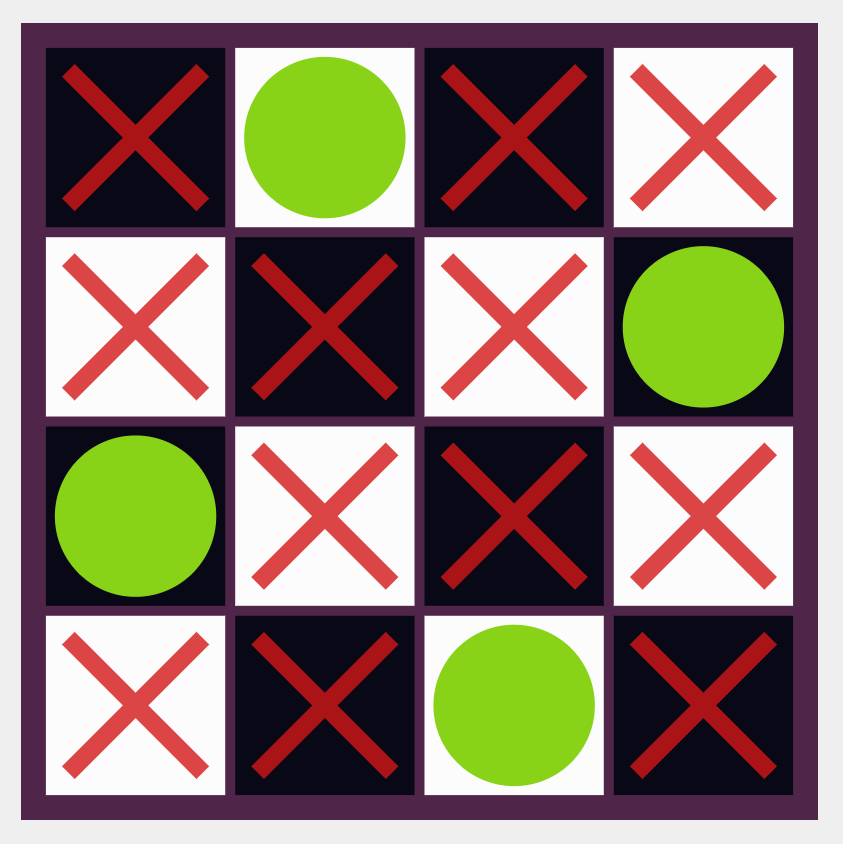
\includegraphics[width=0.7\textwidth]{img/Proof_Chessboard}
  \caption{Final Solution for 4-Queens Problem with Seed \enquote{Exmatrikulator}}
  \label{fig:design}
\end{figure}

Thus it is possible to replicate a certain result as often as possible and at any time. Thus the requirement is considered fulfilled.

\paragraph{Visualization of current progress}
The criterion here was to display the current solution process as a visual representation on the chessboard and as calculation steps. On the user interface, the animation is displayed visually in the middle of the chessboard and the calculations are shown in a box to the right. It should also be mentioned that this can either be done automatically or step by step with a single push of a button. The step size can also be adjusted. You can choose between Micro and Macro. Thus this requirement is also fulfilled.

\paragraph{Pausable Progress}
The requirement was that the simulation could be paused. If the user pressed the \enquote{Play} button, the simulation starts and at the same time the start button turns into a \enquote{Stop} button. This button can be used to stop the animation by pressing it. Please note, however, that the simulation only stops after the current calculation step has been completed. After this has been stopped, the button changes back to \enquote{Play} and the animation can be continued at the corresponding position.

\section{Conclusion}
\label{sec:proConclusion}
As shown in the previous section, this program meets all previously defined requirements. The program is considered successful and the project can now be completed satisfactorily. In summary, it was a very exciting project with no significant problems. Again and again during the implementation phase, the requirements had to be re-examined and decisions had to be made with the help of these decisions. The program had to be easy to use and understand at all times. Both usability and user experience played a role in all areas of the development process. 

The use of Javascript made web development a lot easier, but there were also some difficulties. But these were solved by helpful libraries and technologies like web workers. 

\section{Outlook}
\label{sec:proOutlook}
% cSpell:disable
%TODO Koen. Du musst sagen, wie man die Berechnung optimieren könnte
%Es gibt immer Bereiche eines Programms, die zukünftig noch verbessert werden können. Beispielsweise könnte die Berechnung der Lösung des N Damen Problems bestimmt noch weiter optimiert werden. Dadurch würde die Performanz eventuell verbessert werden, da vor allem bei großen Zahlen für N die Berechnung sehr lange dauert. 
%TODO Koen: durchlesen und eventuell ergänzen
%Eine weitere Idee zur zukünftigen Weiterentwicklung wäre die Verwendung dieses Programms für weitere aussagelogische Probleme und nicht nur das N Damen Problem. Durch die Verwendung der web worker wäre dies durch aus denkbar und umsetzbar. Somit ist der Davis Putman Algorithmus in diesem Programm universell einsetzbar.
%There are always areas of a program that can be improved in the future. For example, the calculation of the solution to the N-Queens Problem could certainly be further optimized. This would possibly improve the performance, because especially with large numbers for N the calculation takes a very long time. 
% cSpell:enable

There are always areas of a program that can be improved in the future for example the performance. But because the program is only used for small numbers of the N-Queens Problem, the speed of the calculations for the larger ones is not the focus for future improvements.  \\
\\
Another idea for future development would be the use of this program for further logical problems and not only the N-Queens Problem. By using the web worker this would be possible. Therefore the Davis Putman algorithm is universally applicable in this program.

%
%    \bibliographystyle{alpha}
%
%    \bibliography{cs}
%
%\end{document}